%%%%%%%% ICML 2022 EXAMPLE LATEX SUBMISSION FILE %%%%%%%%%%%%%%%%%

\documentclass[nohyperref]{article}

% Recommended, but optional, packages for figures and better typesetting:
\usepackage{xcolor}
\usepackage{microtype}
\usepackage{graphicx}
\usepackage{subfigure}
\usepackage{booktabs} % for professional tables
\usepackage{tcolorbox}
\usepackage{listings}
\usepackage{xspace}
\lstset{
basicstyle=\scriptsize\ttfamily,
frame=single,
backgroundcolor=\xcolor{light-gray}
}
% hyperref makes hyperlinks in the resulting PDF.
% If your build breaks (sometimes temporarily if a hyperlink spans a page)
% please comment out the following usepackage line and replace
% \usepackage{icml2022} with \usepackage[nohyperref]{icml2022} above.
\usepackage{hyperref}


% Attempt to make hyperref and algorithmic work together better:
\newcommand{\theHalgorithm}{\arabic{algorithm}}

% Use the following line for the initial blind version submitted for review:
%\usepackage{icml2022}

% If accepted, instead use the following line for the camera-ready submission:
\usepackage[accepted]{icml2022}

% For theorems and such
\usepackage{amsmath}
\usepackage{amssymb}
\usepackage{mathtools}
\usepackage{amsthm}
\usepackage{listings}
\usepackage{comment}

% if you use cleveref..
\usepackage[capitalize,noabbrev]{cleveref}

\usepackage{tikz}
\usetikzlibrary{bayesnet}

% \lstdefineformat{R}{~=\( \sim \)}

%%%%%%%%%%%%%%%%%%%%%%%%%%%%%%%%
% Technical terms
%%%%%%%%%%%%%%%%%%%%%%%%%%%%%%%%
\newcommand{\cascade}{cascade\xspace}
\newcommand{\cascades}{cascades\xspace}
\newcommand{\Cascades}{Cascades\xspace}

%%%%%%%%%%%%%%%%%%%%%%%%%%%%%%%%
% THEOREMS
%%%%%%%%%%%%%%%%%%%%%%%%%%%%%%%%
\theoremstyle{plain}
\newtheorem{theorem}{Theorem}[section]
\newtheorem{proposition}[theorem]{Proposition}
\newtheorem{lemma}[theorem]{Lemma}
\newtheorem{corollary}[theorem]{Corollary}
\theoremstyle{definition}
\newtheorem{definition}[theorem]{Definition}
\newtheorem{assumption}[theorem]{Assumption}
\theoremstyle{remark}
\newtheorem{remark}[theorem]{Remark}

% Todonotes is useful during development; simply uncomment the next line
%    and comment out the line below the next line to turn off comments
%\usepackage[disable,textsize=tiny]{todonotes}
\usepackage[textsize=tiny]{todonotes}

\DeclareMathOperator*{\argmax}{\arg\!\max}

% The \icmltitle you define below is probably too long as a header.
% Therefore, a short form for the running title is supplied here:
\icmltitlerunning{Language Model Cascades}

\begin{document}

\twocolumn[
% \icmltitle{Language Models are Probabilistic Inference Programs}
\icmltitle{Language Model Cascades}
% \icmltitle{Probabilistic Inference over Language Model Programs}

% It is OKAY to include author information, even for blind
% submissions: the style file will automatically remove it for you
% unless you've provided the [accepted] option to the icml2022
% package.

% List of affiliations: The first argument should be a (short)
% identifier you will use later to specify author affiliations
% Academic affiliations should list Department, University, City, Region, Country
% Industry affiliations should list Company, City, Region, Country

% You can specify symbols, otherwise they are numbered in order.
% Ideally, you should not use this facility. Affiliations will be numbered
% in order of appearance and this is the preferred way.
\icmlsetsymbol{equal}{*}

\begin{icmlauthorlist}
\icmlauthor{David Dohan}{comp}
\icmlauthor{Winnie Xu}{comp}
\icmlauthor{Aitor Lewkowycz}{x}
\icmlauthor{Jacob Austin}{comp}
\icmlauthor{David Bieber}{comp}
\icmlauthor{Raphael Gontijo Lopes}{comp}
\icmlauthor{Yuhuai Wu}{comp}
\icmlauthor{Henryk Michalewski}{comp}
\icmlauthor{Rif A. Saurous}{comp}
\icmlauthor{Jascha Sohl-dickstein}{comp}
\icmlauthor{Kevin Murphy}{comp}
\icmlauthor{Charles Sutton}{comp}
\end{icmlauthorlist}

\icmlaffiliation{comp}{Google Research, Mountain View, United States}
\icmlaffiliation{x}{Alphabet, X, the Moonshot Factory}
% \icmlaffiliation{research}{Google Research, Mountain View, United States}

\icmlcorrespondingauthor{David Dohan}{david@ddohan.com}
\icmlcorrespondingauthor{Winnie Xu}{winniexu@cs.toronto.edu}

% You may provide any keywords that you
% find helpful for describing your paper; these are used to populate
% the "keywords" metadata in the PDF but will not be shown in the document
\icmlkeywords{Machine Learning, ICML}

\vskip 0.3in
]

\newcommand{\ddohan}[1]{\textcolor{green}{{[david: #1]}}}
\newcommand{\xwinxu}[1]{\textcolor{purple}{{[winnie: #1]}}}
\newcommand{\kevin}[1]{\textcolor{red}{{[kevin: #1]}}}
\newcommand{\rif}[1]{\textcolor{brown}{{[rif: #1]}}}
\newcommand{\aitor}[1]{\textcolor{cyan}{[aitor: #1]}}
\newcommand{\henryk}[1]{\textcolor{orange}{[henryk: #1]}}
\newcommand{\charles}[1]{\textcolor{purple}{[charles: #1]}}

\urlstyle{same}

% this must go after the closing bracket ] following \twocolumn[ ...

% This command actually creates the footnote in the first column
% listing the affiliations and the copyright notice.
% The command takes one argument, which is text to display at the start of the footnote.
% The \icmlEqualContribution command is standard text for equal contribution.
% Remove it (just {}) if you do not need this facility.


\printAffiliationsAndNotice{}  % leave blank if no need to mention equal contribution
%\printAffiliationsAndNotice{\icmlEqualContribution} % otherwise use the standard text.

% TODOs:
% \begin{itemize}
% % \item Tikz imag of the QTA case, with plate notation to demonst
% % \item Verifiers illustration
% % \item Settle on graphical notation (ladder? compressed ladder?)
% %\item Tool use illustration
% %\item Discuss masked modeling
% %\item Expand appendix
% \end{itemize}

\begin{abstract}
Prompted models have demonstrated impressive few-shot learning abilities.
Repeated interactions at test-time with a single model, or the composition of multiple models together, further expands capabilities. These compositions are probabilistic models, and may be expressed in the language of graphical models with random variables whose values are complex data types such as strings. Cases with control flow and dynamic structure require techniques from probabilistic programming, 
which allow implementing disparate model structures and inference strategies in a unified language.
We formalize several existing techniques from this perspective, including scratchpads / chain of thought, verifiers, STaR, selection-inference, and tool use. We refer to the resulting programs as \emph{language model \cascades}.
%Furthermore, the few shot learning abilities of large language models may be used to amortize inference across tasks.
\end{abstract}

\section{Introduction}
%
Neural network (NN) learning has underpinned state of the art empirical
results in numerous applied machine learning tasks (see for
instance~\cite{krizhevsky2012imagenet,lecun2015deep}). Nonetheless, neural
network learning remains rather poorly understood in several regards.
Notably, it remains unclear why training algorithms find good weights, how
learning is impacted by the network architecture and activations, what is
the role of random weight initialization, and how to choose a concrete
optimization procedure for a given architecture.

We start by analyzing the expressive power of NNs subsequent to the random
weight initialization. The motivation is the empirical success of training
algorithms despite inherent computational intractability, and the fact that
they optimize highly non-convex objectives with potentially many local minima.
Our key result shows that random initialization already positions learning
algorithms at a good starting point. We define an object termed a {\em
computation skeleton} that describes a distilled structure of feed-forward
networks. A skeleton induces a family of network architectures along with a
hypothesis class $\ch$ of functions obtained by certain non-linear
compositions according to the skeleton's structure.  We show that the
representation generated by random initialization is sufficiently rich to
approximately express the functions in $\ch$. Concretely, all functions in
$\ch$ can be approximated by tuning the weights of the last layer, which is
a convex optimization task.

In addition to explaining in part the success in finding good weights, our
study provides an appealing perspective on neural network learning.  We
establish a tight connection between network architectures and their dual
kernel spaces. This connection generalizes several previous constructions
(see Sec~\ref{sec:related}). As we demonstrate, our dual view gives rise to
design principles for NNs, supporting current practice and suggesting
new ideas. We outline below a few points.

\begin{itemize}

\item Duals of convolutional networks appear a more suitable fit for
	vision and acoustic tasks than those of fully connected networks.

\item Our framework surfaces a principled initialization scheme. It is
	very similar to common practice, but incorporates a small correction.

\item By modifying the activation functions, two consecutive fully connected
	layers can be replaced with one while preserving the network's dual kernel.

\item The ReLU activation, i.e. $x \mapsto \max(x,0)$, possesses favorable
	properties. Its dual kernel is expressive, and it can be well approximated by
	random initialization, even when the initialization's scale is moderately
	changed.

\item As the number of layers in a fully connected network becomes very
	large, its dual kernel converges to a degenerate form for any non-linear
	activation.

\item Our result suggests that optimizing the weights of the last layer can
	serve as a convex proxy for choosing among different architectures prior
	to training. This idea was advocated and tested empirically
	in~\cite{saxe2011random}.

\end{itemize}

\vspace{-5pt}
\section{Related Work}
\label{sec:related}
\vspace{-8pt}
\noindent\textbf{Self-Supervised Learning.} 
Recent SSL approaches have shown performance comparable to their supervised learning equivalents~\cite{caron2020unsupervised, caron2021emerging, chen2020simple, he2020momentum, grill2020bootstrap, zbontar2021barlow, bardes2021vicreg, chen2020improved}. In a nutshell, most of these methods use image augmentation techniques to generate correlated views (positives) from a sample, and then learn a model that is invariant to these augmentations by enforcing the network to output similar representations for the positives. Initially, contrastive learning, based on instance discrimination~\cite{wu2018unsupervised} using noise-contrastive estimation~\cite{gutmann2010noise, oord2018representation}, was a popular strategy~\cite{chen2020simple, he2020momentum}. However, this learning paradigm 
requires large batch sizes or memory banks. A few methods that use a negative-free cosine similarity loss~\cite{grill2020bootstrap, chen2021exploring} have addressed such issues.

Concurrently, clustering-based methods (SwAV~\cite{caron2020unsupervised}, DeepCluster v2~\cite{caron2020unsupervised, caron2018deep} and DINO~\cite{caron2021emerging}) have also been proposed. They do not operate on the features directly, and instead compare positives through a cross-entropy loss using cluster prototypes as a proxy. Redundancy reduction-based methods have also been popular\cite{ermolov2021whitening, zbontar2021barlow, bardes2021vicreg}. Among them, BarlowTwins \cite{zbontar2021barlow} considers an objective function measuring the cross-correlation matrix between the features, and VicReg\cite{bardes2021vicreg} uses a mix of variance, invariance and covariance
regularizations. Methods such as~\cite{dwibedi2021little} have explored the use of nearest-neighbour retrieval and divide and conquer~\cite{tian2021divide}. However, none of these works studied the ability of SSL methods to learn continually and adaptively.


\noindent\textbf{Continual Learning.} A plethora of methods have been developed to counteract catastrophic forgetting~\cite{kirkpatrick2017overcoming, Rusu16progressive, shin2017continual, Lopez-Paz17, Chaudhry19, serra2018overcoming, chaudhry2018riemannian, Aljundi17, Zenke17, buzzega2020dark, fini2020online, douillard2020podnet, wu2019large, castro2018end, rebuffi2017icarl, hou2019learning, prabhu2020gdumb, Li17learning, ostapenko2019learning, cha2021co2l, Robins95}. Following~\cite{de2019continual}, these works can be organized into three macro-categories: replay-based~\cite{ostapenko2019learning, Robins95, rebuffi2017icarl, buzzega2020dark, Chaudhry19, Lopez-Paz17}, regularization-based~\cite{fini2020online, Li17learning, shin2017continual, kirkpatrick2017overcoming, Zenke17, Aljundi17, castro2018end, douillard2020podnet, hou2019learning, chaudhry2018riemannian, wu2019large, cha2021co2l}, and parameter isolation
methods~\cite{Rusu16progressive, serra2018overcoming}. All these works evaluate the effectiveness of CL methods using a linear classifier learned
sequentially over time. However, this evaluation does not reflect an important aspect, \textit{i.e.}, the internal dynamics of the hidden representations. Moreover, most CL methods tend to rely on supervision in order to mitigate catastrophic forgetting. A few of them can be adapted for the unsupervised setting, although their effectiveness is greatly reduced (see discussion in Sec.~\ref{sec:cassowary}, Sec.~\ref{sec:experiments} and the supplementary material). 

Works such as~\cite{rao2019continual, achille2018life, smith2019unsupervised} laid the foundations of unsupervised CL, but their studies are severely limited to digit-like datasets, \emph{e.g.}, MNIST and Omniglot, and the proposed methods are unfit for large-scale scenarios. Recently, \cite{gallardo2021self, caccia2021special} explored self-supervised pretraining for supervised continual learning with online and few-shot tasks, and \cite{cha2021co2l} presented a supervised contrastive CL approach. Two concurrent works~\cite{lin2021continual, madaan2021rethinking} have also attempted to address CSSL recently. The former~\cite{lin2021continual} extends~\cite{cha2021co2l} to the unsupervised setting, but is specifically designed for contrastive SSL, such as~\cite{chen2020simple,he2020momentum}, and lacks generalizability to other popular SSL paradigms. The latter~\cite{madaan2021rethinking} is also limited as it only shows small-scale experiments in the class-incremental setting and considers just two SSL methods. In contrast, we present a general framework for CSSL with superior performance, conduct large-scale experiments on three challenging settings, thereby presenting a deeper analysis of CSSL.
\section{\Cascades}

In this section, we show how to create
\cascades\ of LMs to tackle various
language-based reasoning problems.
A \emph{\cascade} is a probabilistic program that includes
string-valued random variables, sampled from an LM.
For example, Figure~\ref{fig:cot_cascade} is a simple \cascade\ for question answering.
%For example, Figure~\ref{fig:si_cascade} is a simple \cascade\ for the selection-inference algorithm.
Each of the \texttt{yield} expressions return a string distributed according to the language model \texttt{S}.\footnote{The first argument
to \texttt{S} defines a unique name for the random variable,
and the remaining arguments conditions the LM on a string prefix. A variable may be marked as observed within the program, \texttt{S('varname', obs='observed value')}, or at inference time} This program defines a joint distribution over the variables \texttt{question, thought}, and \texttt{answer}.  Programs with complex control flow and observations are included in Appendix~\ref{app:implementation}.

We implement \cascades\ as a trace-based probabilistic programming language embedded in Python via effect handlers, inspired by \citet{pyro, numpyro}, and via coroutines, inspired by \citet{pymc4}. A pretrained LM is used to parameterize all conditional distributions. A \cascade supports arbitrary control flow and recursion. While the current presentation is in terms of few-shot prompting of causal language models, we emphasize that the ideas are immediately applicable to finetuned models, masked LM setting, and other complex data types including images.

\subsection{Scratchpads and Chain of thought}
\label{sec:QTA}

As our first example, we show how to 
 represent a chain of thought \citep{scratchpads, chainofthought} as shown in 
\cref{fig:QTA} and subsequent graphical model figures; refer to the corresponding probabilistic programs in \cref{app:implementation}.
We condition the $A$ node not just on the test question $Q$,
but also on previous $(Q^m,T^m,A^m)$ triples, which 
constitute the few-shot prompting part of the model.
This is denoted by the shaded nodes inside the plate.
Inference can be implemented by ancestral
sampling.

%
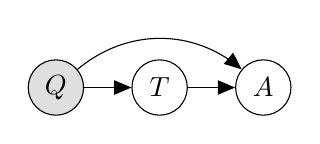
\begin{tikzpicture}
  % Define nodes
  \node[obs]           (Q) {$Q$};
  \node[latent, right=0.6cm of Q]         (T) {$T$};
  \node[latent, right=0.6cm of T]         (A) {$A$};

  % Connect the nodes
  \edge {Q} {T} ; %
  \edge {T} {A} ; %
  \draw [->] (Q) to [out=40,in=140] (A);
%   \path[every node/.style={font=\sffamily\small}]
%     (Q) edge[bend right] node [left] {} (A);
%   \edge[bend right=30] {Q} {A} ; %
\end{tikzpicture}
\begin{figure}[h!]
\centering
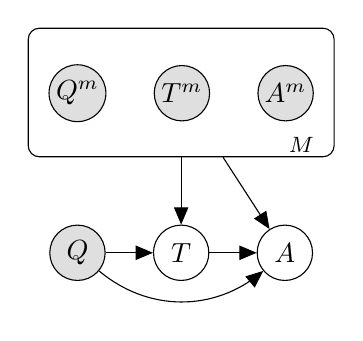
\begin{tikzpicture}
  % notation
  % [positioning] (name) {displayed name}
  

% Plate  
% Define nodes
\node[obs]           (Qf) {$Q^m$};
\node[obs, right=0.6cm of Qf]         (Tf) {$T^m$};
\node[obs, right=0.6cm of Tf]         (Af) {$A^m$};
%
%  % Connect the nodes
% \edge {Qf} {Tf} ; %
% \edge {Tf} {Af} ; %
% \draw [->] (Qf) to [out=40,in=140] (Af);
%  
\plate [inner sep=.25cm,yshift=.2cm] {fewshot} {(Qf)(Tf)(Af)} {$M$};

% Target task
%\node[obs]           (Q) {$Q$};
 \node[obs, below=1.3cm of Qf]           (Q) {$Q$};
\node[latent, right=0.6cm of Q]         (T) {$T$};
\node[latent, right=0.6cm of T]         (A) {$A$};
\edge {Q} {T} ; %
\edge {T} {A} ; %
\draw [->] (Q) to [out=-40,in=-140] (A);
  
  
% Connect plate to the 
\edge {fewshot} {T};
\edge {fewshot} {A};
\end{tikzpicture}
\caption{Question-Thought-Answer model.}
\label{fig:QTA}
\end{figure}



%In \cascades, we define the model in code in Figure~\ref{fig:cot_cascade}, where S is a (conditional) string distribution.
%The prompt for each variable is automatically constructed at inference time based on input variables and few shot examples.

% \charles{The program should not sample $q$, should it? Would it be more clear to leave off the 'question' etc arguments? Perhaps instead of question=q, we should use prefix=q, prefix=concat(q, t) to make it more generic? If we say this is a PPL, the reader is going to wonder whether we have observes. The program also does not explain how the prompt examples are used.}

% david: We can either say `S('question', obs='the question')`, or have the inference call inject the value (which is what I do in practice):
% `infer(program, observe(question='the question')`

% charles: Sure, the infer way is fine.  

% charles: I guess we can explain in the text that the first argument to S is a name for the r.v.

 % q = yield S('question')
  
\begin{figure}[h]
\begin{verbatim}
def qta():
  q = yield S('question')
  t = yield S('thought', question=q)
  a = yield S('answer', question=q, 
                        thought=t)
  return a
\end{verbatim}
\caption{Chain of thought \cascade\ in Python. Each \texttt{yield S(...)} statement samples a string from an LM. The name of the random variable is provided as the first argument to \texttt{S}.}
\label{fig:cot_cascade}
\end{figure}  

\subsection{Semi-supervised learning}
\label{sec:STAR}
In \cref{sec:QTA}, we provided a manually created set  $(Q^m,T^m,A^m)$ triples,
where the ``thoughts'' or ``rationalizations'' were provided.
A more scalable approach is to define a small set $D_S$
of such ``supervised'' triples,
but then to provide a larger set $D_L$ of $(Q^m,A^m)$ pairs,
which are easier to gather. % (e.g., by scraping question-answering web-sites).
We can augment the pairs in $D_L$ by adding 
the hidden $T^m$ variable to get a semi-supervised setup, shown in  
\cref{fig:QTAhidden}.

\begin{figure}[h!]
\centering
\begin{tikzpicture}
  % notation
  % [positioning] (name) {displayed name}
  
% Target task
\node[obs, below=0.8cm of fewshot]           (Q) {$Q$};
\node[latent, right=0.6cm of Q]         (T) {$T$};
\node[latent, right=0.6cm of T]         (A) {$A$};
\edge {Q} {T} ; %
\edge {T} {A} ; %
\draw [->] (Q) to [out=-40,in=-140] (A);
  
% Plate  
% Define nodes
\node[obs]           (Qf) {$Q^m$};
\node[latent, right=0.6cm of Qf]         (Tf) {$T^m$};
\node[obs, right=0.6cm of Tf]         (Af) {$A^m$};
%
%  % Connect the nodes
 \edge {Qf} {Tf} ; %
 \edge {Tf} {Af} ; %
% \draw [->] (Qf) to [out=40,in=140] (Af);
%  
\plate [inner sep=.25cm,yshift=.2cm] {fewshot} {(Qf)(Tf)(Af)} {$M$};

% Connect plate to the 
\edge {fewshot} {T};
\edge {fewshot} {A};
\end{tikzpicture}
\caption{QTA model with hidden thoughts.}
\label{fig:QTAhidden}
\end{figure}


The Self-Taught Reasoner (STaR) \citep{zelikman2022star} proposes a procedure for fine-tuning LMs in the chain-of-thought type setting.
We can interpret their method as a stochastic EM-like procedure in the cascade of \cref{fig:QTAhidden}.
In particular, they first fine-tune on the ``fully observed''
dataset $D_S = \{(Q^m,T^m,A^m)\}$.
Then they impute the unknown $T_i$ values in the 
``partially observed'' dataset  $D_L = \{(Q^m,T^m=?,A^m)\}$
during the ``E'' step by doing rejection sampling on $p(T, A | Q^m)$ until finding a thought which leads to the known correct answer. If sampling $(T,A)$ given the question fails to find the correct answer, they sample thoughts from $p(T | Q^m, A^m)$. This uses a recognition network to approximately sample from the posterior distribution over thoughts given the known correct answer.
%where the true answer is added to the prompt.
They call this approach  ``rationale generation with rationalization''. They then update the parameters in the ``M'' step based on these imputed thoughts.
By interpreting the rationale generation at this higher level of abstraction, we open up the possibility of applying this tuning method to other types of cascades.


%See \cref{sec:STAR} for details.

% We can fine-tune the model on this semi-supervised data
% using an EM-like procedure,
% as proposed for STaR (self-taught reasoner) \citep{zelikman2022star}.
% In the E step, they impute the unknown $T^m$ values in the $D_L$
% dataset, and in the M step, they update the LM parameters.
% 
% In the E step, thoughts are imputed by sampling from 
% $p(T | Q^m, A=A^m)$ using rejection sampling,
% where $p$ represents the language model,
% and they use $p(T,A|Q^m)$ as the proposal.
% If this fails to yield any correct answers,
% they use a more powerful proposal, 
%  $p(T,A|Q^m,A^m)$,
%  where the true answer is added to the prompt.
% They call this approach 
% ``rationale generation with rationalization''

%\input{star-old}

\subsection{Selection-Inference}
\label{sec:selection_inference}

Selection Inference \citep{selection_inference} is a recent example of multiple interacting LM modules. It proposes splitting reasoning into: the \textit{selection} module which selects a subset of facts given a question, and the \textit{inference} module which infers new facts given this subset.
%See \cref{sec:selection_inference} for details.

It may be represented by the model in \cref{fig:selective}. Here $S$ is the selection of a subset of ``facts''
from a pre-specified set of facts,
and $I$ is an inference driven by that fact.
The $S$ and $I$ nodes
can be iterated to do multistep reasoning.
The model is ``trained'' by giving it examples,
$D = \{ (Q^m, \{F^{mj}\}, S^m, I^m, A^m): m=1:M\}$,
as part of the prompt.
% It is then given a test question,
% and the answer is computed using
% $A \sim p(A|Q,D)$,
% ignoring (``marginalizing out'')\todo{ddohan: is this actually marginalizing out? It's just taking a single monte carlo sample by default. I would expect > 1 sample to marginalize}
% any intermediate $S$ or $I$ strings that
% might be generated by the model.

\begin{figure}[h!]
\centering
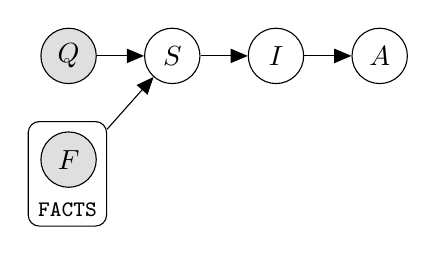
\begin{tikzpicture}
  % Define nodes
  \node[obs]           (Q) {$Q$};
  \node[obs, below=0.6cm of Q]           (F) {$F$};
  \plate{Fs} {
      (F)
  } {\texttt{FACTS}} %{$F \in \text{\texttt{FACTS}}$}
  \node[latent, right=0.6cm of Q]         (S) {$S$};
  \node[latent, right=0.6cm of S]         (I) {$I$};
  \node[latent, right=0.6cm of I]         (A) {$A$};

  % Connect the nodes
  \edge {Q,Fs} {S} ; %
  \edge {S} {I} ; %
  \edge {I} {A} ; %
  %\draw [->] (Q) to [out=40,in=140] (I);
  %\draw [->] (Q) to [out=40,in=140] (A);
%  \draw [->] (S) to [out=40,in=140] (A);
\end{tikzpicture}
\caption{Selection inference as a cascade. Here $S$ is the selected subset of facts and $I$ is an inference driven by this subset.}
\label{fig:selective}
\end{figure}

\subsection{Verifiers}
\label{sec:verifiers}

Although adding explicit ``thought'' variables to a model
has been found to improve performance, models still arrive at incorrect answers, or the correct answer for an erroneous reason.
An intuitive way to improve model performance is to train it to judge whether an answer and thought are likely to be ``valid''. \citet{verifiers} propose using a separate model as a verifier to filter solutions to reasoning tasks.
%sometimes
%these ``thoughts'' are erroneous,
%even though the answer may be correct.

We can create a ``labeled'' training
set of the form
$D = \{ (Q^m, T^m, A^m, V^m\}$,
where we add a ``verification'' label 
$V^m \in \{0, 1 \}$,
representing whether the thought $T^m$
is a valid form of reasoning for deriving
$A^m$ from $Q^m$, and $A^m$ is the correct answer.
This can be particularly helpful in settings
where there may be more than one way of deriving
the answer. The verifiers may be used to reject incorrect examples in ancestral sampling, and the thought generator may itself be conditioned on the verifiers being correct by finetuning or prompting, reminiscent of RL as inference \cite{rl_inference} and goal-conditioned policies such as decision-transformer \cite{decision_transformer}.

%\begin{figure}[h!]
\centering
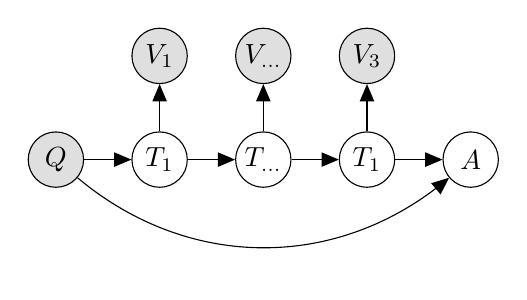
\begin{tikzpicture}
  % Define nodes
  \node[obs]           (Q) {$Q$};
  \node[latent, right=0.6cm of Q]         (T1) {$T_1$};
  \node[latent, right=0.6cm of T1]         (T2) {$T_{...}$};
  \node[latent, right=0.6cm of T2]         (T3) {$T_1$};
  \node[latent, right=0.6cm of T3]         (A) {$A$};
  
  \node[obs, above=0.6cm of T1]         (V1) {$V_1$};
  \node[obs, above=0.6cm of T2]         (V2) {$V_{...}$};
  \node[obs, above=0.6cm of T3]         (V3) {$V_3$};

  % Connect the nodes
  \edge {Q} {T1} ; %
  \edge {T1} {T2} ; %
  \edge {T2} {T3} ; %
  \edge {T3} {A} ; %
  \edge {T1} {V1} ; %
  \edge {T2} {V2} ; %
  \edge {T3} {V3} ; %
  \draw [->] (Q) to [out=-40,in=-140] (A);
%   \path[every node/.style={font=\sffamily\small}]
%     (Q) edge[bend right] node [left] {} (A);
%   \edge[bend right=30] {Q} {A} ; %
\end{tikzpicture}
\caption{The current way in which verifiers are diagrammed. Note that every node actually gets as input the concatenated strings of all of its parent nodes.}
\label{fig:verifier}
\end{figure}



%

\begin{figure}[h!]
\centering
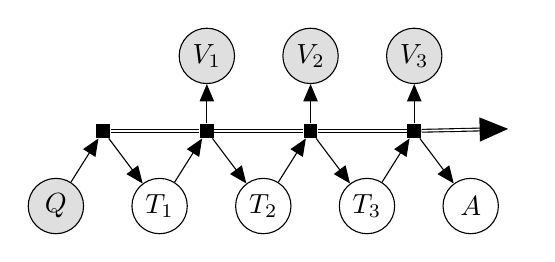
\begin{tikzpicture}
  % Define nodes
  \node[obs]    at (0,0)       (Q) {$Q$};

  \node[latent, right=0.6cm of Q]         (T1) {$T_1$};
  \node[latent, right=0.6cm of T1]         (T2) {$T_2$};
  \node[latent, right=0.6cm of T2]         (T3) {$T_3$};
  \node[latent, right=0.6cm of T3]         (A) {$A$};
  
  \node[factor, above=0.5cm of Q, xshift=0.6cm]       (stream1) {};
  \node[factor, above=0.5cm of T1, xshift=0.6cm]       (stream2) {};
  \node[factor, above=0.5cm of T2, xshift=0.6cm]       (stream3) {};
  \node[factor, above=0.5cm of T3, xshift=0.6cm]       (stream4) {};
  \node[above=0.5cm of A, xshift=0.6cm]       (stream5) {};
  
  \node[obs, above=0.5cm of stream2]         (V1) {$V_1$};
  \node[obs, above=0.5cm of stream3]         (V2) {$V_2$};
  \node[obs, above=0.5cm of stream4]         (V3) {$V_3$};


  % Connect the nodes
  \edge {Q} {stream1} ; %
  \edge {T1} {stream2} ; %
  \edge {T2} {stream3} ; %
  \edge {T3} {stream4} ; %
  \edge {stream1} {T1} ; %
  \edge {stream2} {T2} ; %
  \edge {stream3} {T3} ; %
  \edge {stream4} {A} ; %
  \draw [double] (stream1) to (stream2);
  \draw [double] (stream2) to (stream3);
  \draw [double] (stream3) to (stream4);
  \draw [double, ->] (stream4) to (stream5);

%   \edge {stream1} {stream2} ; %
%   \edge {stream2} {stream3} ; %
%   \edge {stream3} {stream4} ; %
%   \edge {stream4} {stream5} ; %
%   \edge {Q} {T1} ; %
%   \edge {T1} {T2} ; %
%   \edge {T2} {T3} ; %
%   \edge {T3} {A} ; %
  \edge {stream2} {V1} ; %
  \edge {stream3} {V2} ; %
  \edge {stream4} {V3} ; %
%   \draw [->] (Q) to [out=-40,in=-140] (A);
%   \path[every node/.style={font=\sffamily\small}]
%     (Q) edge[bend right] node [left] {} (A);
%   \edge[bend right=30] {Q} {A} ; %
\end{tikzpicture}
\caption{A proposed alternate diagram for verifiers. The double line indicates a text stream, or text buffer. Arrows entering the double line are appended to the buffer. Arrows exiting the line read out the entirety of the buffer at that point.}
\label{fig:verifier}
\end{figure}
%


\begin{figure}[h!]
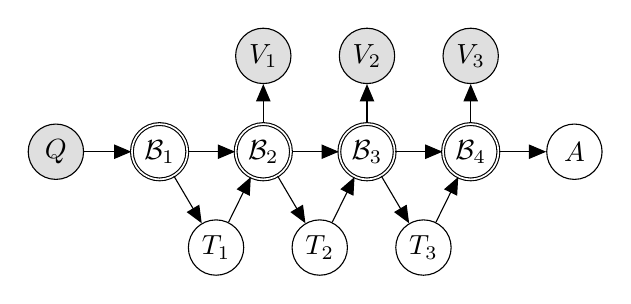
\begin{tikzpicture}
  % Define nodes

  \node[latent]         (T1) {$T_1$};
  \node[latent, right=0.6cm of T1]         (T2) {$T_2$};
  \node[latent, right=0.6cm of T2]         (T3) {$T_3$};
  
%   \node[latent, double, above=0.5cm of Q, xshift=0.6cm]       (stream1) {$\mathcal B_1$};
  \node[latent, double, above=0.5cm of T1, xshift=0.6cm]       (stream2) {$\mathcal B_2$};
  \node[latent, double, left=0.6cm of stream2]       (stream1) {$\mathcal B_1$};
  \node[latent, double, above=0.5cm of T2, xshift=0.6cm]       (stream3) {$\mathcal B_3$};
  \node[latent, double, above=0.5cm of T3, xshift=0.6cm]       (stream4) {$\mathcal B_4$};
%   \node[above=0.5cm of A, xshift=0.6cm]       (stream5) {};

  \node[obs, left=0.6cm of stream1]       (Q) {$Q$};

  
  \node[obs, above=0.5cm of stream2]         (V1) {$V_1$};
  \node[obs, above=0.5cm of stream3]         (V2) {$V_2$};
  \node[obs, above=0.5cm of stream4]         (V3) {$V_3$};

  \node[latent, right=0.6cm of stream4]         (A) {$A$};


  % Connect the nodes
  \edge {Q} {stream1} ; %
  \edge {T1} {stream2} ; %
  \edge {T2} {stream3} ; %
  \edge {T3} {stream4} ; %
  \edge {stream1} {T1} ; %
  \edge {stream2} {T2} ; %
  \edge {stream3} {T3} ; %
  \edge {stream4} {A} ; %
  \edge {stream1} {stream2};
  \edge {stream2} {stream3};
  \edge {stream3} {stream4};
%   \draw [double] (stream1) to (stream2);
%   \draw [double] (stream2) to (stream3);
%   \draw [double] (stream3) to (stream4);
%   \draw [double, ->] (stream4) to (stream5);

%   \edge {stream1} {stream2} ; %
%   \edge {stream2} {stream3} ; %
%   \edge {stream3} {stream4} ; %
%   \edge {stream4} {stream5} ; %
%   \edge {Q} {T1} ; %
%   \edge {T1} {T2} ; %
%   \edge {T2} {T3} ; %
%   \edge {T3} {A} ; %
  \edge {stream2} {V1} ; %
  \edge {stream3} {V2} ; %
  \edge {stream4} {V3} ; %
%   \draw [->] (Q) to [out=-40,in=-140] (A);
%   \path[every node/.style={font=\sffamily\small}]
%     (Q) edge[bend right] node [left] {} (A);
%   \edge[bend right=30] {Q} {A} ; %
\end{tikzpicture}
\caption{Verifier model.
The deterministic $B_t$ nodes are buffer nodes
that accumulate all the past strings.
All other nodes are stochastic.
}
\label{fig:verifier}
\end{figure}








\begin{figure}[h!]
\centering
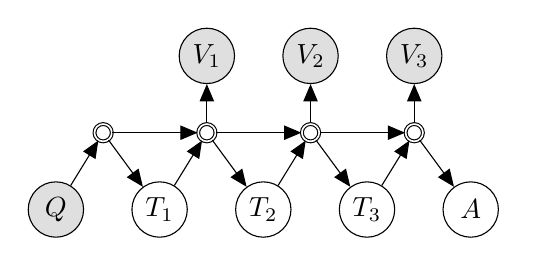
\begin{tikzpicture}
  % Define nodes
  \node[obs]    at (0,0)       (Q) {$Q$};

  \node[latent, right=0.6cm of Q]         (T1) {$T_1$};
  \node[latent, right=0.6cm of T1]         (T2) {$T_2$};
  \node[latent, right=0.6cm of T2]         (T3) {$T_3$};
  \node[latent, right=0.6cm of T3]         (A) {$A$};
  
  \node[latent, double, minimum size=0.22cm, above=0.5cm of Q, xshift=0.6cm]       (stream1) {};
  \node[latent, double, minimum size=0.22cm, above=0.5cm of T1, xshift=0.6cm]       (stream2) {};
  \node[latent, double, minimum size=0.22cm, above=0.5cm of T2, xshift=0.6cm]       (stream3) {};
  \node[latent, double, minimum size=0.22cm, above=0.5cm of T3, xshift=0.6cm]       (stream4) {};
  \node[right=0.4cm of stream4, xshift=0.6cm]       (stream5) {};
  
  \node[obs, above=0.5cm of stream2]         (V1) {$V_1$};
  \node[obs, above=0.5cm of stream3]         (V2) {$V_2$};
  \node[obs, above=0.5cm of stream4]         (V3) {$V_3$};


  % Connect the nodes
  \edge {Q} {stream1} ; %
  \edge {T1} {stream2} ; %
  \edge {T2} {stream3} ; %
  \edge {T3} {stream4} ; %
  \edge {stream1} {T1} ; %
  \edge {stream2} {T2} ; %
  \edge {stream3} {T3} ; %
  \edge {stream4} {A} ; %
%   \draw (stream1) to (stream2);
%   \draw (stream2) to (stream3);
%   \draw (stream3) to (stream4);
%   \draw [double, ->] (stream4) to (stream5);

  \edge {stream1} {stream2};
  \edge {stream2} {stream3};
  \edge {stream3} {stream4};
 % \edge {stream4} {stream5};
 
%   \edge {stream1} {stream2} ; %
%   \edge {stream2} {stream3} ; %
%   \edge {stream3} {stream4} ; %
%   \edge {stream4} {stream5} ; %
%   \edge {Q} {T1} ; %
%   \edge {T1} {T2} ; %
%   \edge {T2} {T3} ; %
%   \edge {T3} {A} ; %
  \edge {stream2} {V1} ; %
  \edge {stream3} {V2} ; %
  \edge {stream4} {V3} ; %
%   \draw [->] (Q) to [out=-40,in=-140] (A);
%   \path[every node/.style={font=\sffamily\small}]
%     (Q) edge[bend right] node [left] {} (A);
%   \edge[bend right=30] {Q} {A} ; %
\end{tikzpicture}
\caption{
Verifier model.
The small double-ringed
nodes are deterministic buffer nodes
that concatenate their inputs, accumulating all past strings.
All other nodes are stochastic. The verifiers are observed to take on the ``correct'' value.
}
\label{fig:verifier}
\end{figure}





We can extend this to  $N$-step reasoning as follows
(where  we drop conditioning on $D$
for brevity):
{\footnotesize
\begin{align*}
p(A|Q,V_{1:N}=1)
&\propto \sum_{T_{1:N}}
p(A,T_{1:N},V_{1:N}=1\,|\,Q),
\end{align*}
}
where
{\footnotesize
\begin{align*}
p(A,T_{1:N},V_{1:N}=1|Q)
&= \left[ \prod_{t=1}^N p(T_t|T_{1:t-1},Q)
p(V_t=1|T_{1:t},Q) \right] \\
& \times p(A|T_{1:N},Q).
\end{align*}
}
\noindent We can represent this 
as shown in \cref{fig:verifier}.
% where the 
% double-ringed nodes are deterministic
% buffer variables that accumulates all the past strings.

% TODO: Clarify this. bpoole didn't get & he understands ladder VAEs well
%(This restores the first-order Markov property,
%and is similar to how RNNs are used
%to define ladder VAEs \citep{Sonderby2016ladder}.)

To see why such a verification model can be useful,
consider (for simplicity) the case where $N=1$.
Suppose we have trained the model to generate valid
thoughts and answers by giving it suitable training examples,
and then we generate $K$ samples
$(T^k,V^k,A^k) \sim p(T,V,A|Q,D)$.
We can then rank the samples for validity by computing
$r^k = p(V^k=1|A^k, Q, D)$,
and then picking the  $A^k$ with largest score $r^k$.

\citet{verifiers} train the verifier to predict a binary correctness label.  \citet{language_feedback} incorporates natural language feedback, and finds that learning is significantly more sample efficient. Preliminary evidence suggests that LMs are capable of critiquing their own chain of reasoning in language, in which case the verifier produces natural language and $p(V_{1:N} = 1 | Q, A, T_{1:N})$ becomes the likelihood of the verifier taking on a particular string value, such as $p(V_{1:N}=\text{"The reasoning and solution are correct."} | ...)$. \citet{openai_critique} study model generated critiques in the context of summarization.

% \ddohan{We view this feedback as an auxiliary variable which can be conditioned to inform inference.}

% \kevin{Should we mention Rapha's preliminary results?}

\begin{comment}
One way to perform inference in this model 
would be to use
particle filtering. The hope is that, by conditioning
on $V_{1:N}=1$,
we increase the probability that the sampled
$T_{1:N}$ values constitute
a valid chain of reasoning
for deriving $A$ from $Q$ and $D$.
This can then provide higher quality training data
in an EM-like fine-tuning scheme, similar
to STaR in \cref{sec:STAR}.
However, we leave evaluation of this idea to future work.
\end{comment}

\subsection{Tool-use}
The applications discussed so far involve iterating a language model, within some control flow, without external feedback. There are many tasks of interest in which a model is interacting with external systems. \citet{verifiers} has an LM use a calculator to solve math tasks, while \citet{webgpt} put an LM in a loop with a web browser to answer questions. Using PPLs to represent these probabilistic models allows easily representing these cases, by writing the call to the external tool, such as the calculator, directly
into the program.
Then techniques from simulation based inference, for example, can be applied to do inference in such situations \cite{simulation_inference}.

\begin{comment}
\charles{Suggest cut for time.}
\kevin{Agreed}
%\begin{tikzpicture}
%  % Define nodes
%  \node[obs]           (Q) {$Q$};
%  \node[latent, right=0.6cm of Q]         (act_1) {$\text{action}_1$};
%  \node[latent, right=0.6cm of Q]         (act_2) {$\text{action}_{...}$};
%  \node[latent, right=0.6cm of Q]         (act_3) {$\text{action}_n$};
%  
%  \node[latent, rectangle]           (env1) {$env_1$};
%  \node[latent, rectangle]           (env2) {$env_2$};
%  \node[latent, rectangle]           (env3) {$env_3$};
%
%  % Connect the nodes
%  %\edge {Q} {T} ; %
%  %\edge {T} {A} ; %
%  %\draw [->] (Q) to [out=40,in=140] (A);
%%   \path[every node/.style={font=\sffamily\small}]
%%     (Q) edge[bend right] node [left] {} (A);
%%   \edge[bend right=30] {Q} {A} ; %
%\end{tikzpicture}
%
\end{comment}
\subsection{Twenty questions}
\label{sec:twenty}

In this section, we discuss experimental results using \cascades\ to solve the
 ``Twenty Questions'' task from BigBench \citep{bigbench}.
This task  involves a conversation between two agents, Alice and Bob.
Both agents are presented with the rules of the game, and Alice is additionally presented with a concept (e.g. `apple') to describe.
Bob has to guess the concept by asking a series of  questions
$B_t$ of the form ``Is it X?'', to which Alice answers
$A_t \in \{ \text{`Yes.'}, \text{`No.'}\}$.
We repeat this process until Bob guesses correctly, or we hit the limit of $T$ rounds.
This can be thought of as a pair of interacting Markov chains, which exchange strings, until some final end state is reached,
 as illustrated in \cref{fig:twenty}.


\begin{figure}[h!]
\centering
% \begin{tikzpicture}
%   % Define nodes
%   \node[obs]    at (0,0)       (C) {\tiny{\texttt{CONCEPT}}};
%   \node[latent, right=1.4cm of C]         (A1) {$A_1$};
%   \node[latent, right=0.9cm of A1]         (A2) {$A_2$};
% %   \node[latent, right=0.6cm of A2]         (A3) {$A_3$};
%   \node[latent, above=0.6cm of A1, xshift=-.8cm]         (B1) {$B_1$};
%   \node[latent, right=0.9cm of B1]         (B2) {$B_2$};
% %   \node[latent, right=0.6cm of B2]         (B3) {$B_3$};

%   \node[obs, left=0.75cm of B1]           (R) {\tiny{\texttt{RULES}}};

%   \node[right=0.3cm of B2] (label1) {\Large\textbf{. . .}};
%   \node[right=0.3cm of A2] (label1) {\Large\textbf{. . .}};


%   % Connect the nodes
%   \edge {R} {B1} ; %
%   \edge {C,R,B1} {A1} ; %
%   \edge {R,A1,B1,B2} {A2} ; %
% %   \edge {A2,B2,B3} {A3} ; %
%   \edge {R} {B1} ; %
%   \edge {A1,B1} {B2} ; %
% %   \edge {A2,B2} {B3} ; %
%   \draw [->] (R) to [out=40,in=140] (B2);
%   \draw [->] (C) to [out=-40,in=-140] (A2);
% %   \draw [->] (Q) to [out=40,in=140] (A);
% %   \draw [->] (S) to [out=40,in=140] (A);
% \end{tikzpicture}

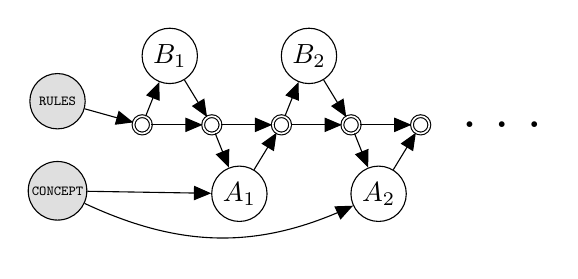
\begin{tikzpicture}
  \node[obs]       (R) {\tiny{\texttt{RULES}}};

  \node[obs, below=0.4cm of R]       (C) {\tiny{\texttt{CONCEPT}}};

% stream
  \node[latent, double, minimum size=0.22cm, right=0.6cm of R, yshift=-0.3cm]       (BS1) {};
  \node[latent, double, minimum size=0.22cm, right=0.65cm of BS1]       (BS2) {};
  \node[latent, double, minimum size=0.22cm, right=0.65cm of BS2]       (BS3) {};
  \node[latent, double, minimum size=0.22cm, right=0.65cm of BS3]       (BS4) {};
  \node[latent, double, minimum size=0.22cm, right=0.65cm of BS4]       (BS5) {};

  \node[latent, above=0.4cm of BS1, xshift=0.35cm]         (B1) {$B_1$};
  \node[latent, above=0.4cm of BS3, xshift=0.35cm]         (B2) {$B_2$};
%   \node[latent, right=0.9cm of B1]         (B2) {$B_2$};

  \node[latent, below=0.4cm of BS2, xshift=0.35cm]         (A1) {$A_1$};
  \node[latent, below=0.4cm of BS4, xshift=0.35cm]         (A2) {$A_2$};


  \node[right=0.3cm of BS5] (label1) {\Large\textbf{. . .}};

    \edge {R} {BS1} ; 
    \edge {BS1} {BS2}; 
    \edge {BS2} {BS3}; 
    \edge {BS3} {BS4}; 
    \edge {BS4} {BS5}; 

    \edge {BS1} {B1} ;
    \edge {B1} {BS2} ;
    \edge {BS2} {A1} ;
    \edge {A1} {BS3} ;
    \edge {BS3} {B2} ;
    \edge {B2} {BS4} ;
    \edge {BS4} {A2} ;
    \edge {A2} {BS5} ;

    \edge {C} {A1} ;
      \draw [->] (C) to [out=-25,in=-155] (A2);


\end{tikzpicture}

% \begin{tikzpicture}

%   \node[obs]    at (0,0)       (C) {\tiny{\texttt{CONCEPT}}};
%   \node[obs, above=0.3cm of C]           (R) {\tiny{\texttt{RULES}}};

% %% alice stream
%   \node[latent, double, minimum size=0.22cm, right=0.6cm of C, yshift=0.15cm]       (AS1) {};
%   \node[latent, double, minimum size=0.22cm, right=0.65cm of AS1]       (AS2) {};
%   \node[latent, double, minimum size=0.22cm, right=0.65cm of AS2]       (AS3) {};
%   \node[latent, double, minimum size=0.22cm, right=0.65cm of AS3]       (AS4) {};
%   \node[latent, double, minimum size=0.22cm, right=0.65cm of AS4]       (AS5) {};

% %% bob stream
%   \node[latent, double, minimum size=0.22cm, above=0.6cm of AS1]       (BS1) {};
%   \node[latent, double, minimum size=0.22cm, right=0.65cm of BS1]       (BS2) {};
%   \node[latent, double, minimum size=0.22cm, right=0.65cm of BS2]       (BS3) {};
%   \node[latent, double, minimum size=0.22cm, right=0.65cm of BS3]       (BS4) {};
%   \node[latent, double, minimum size=0.22cm, right=0.65cm of BS4]       (BS5) {};

%   \node[latent, above=0.4cm of BS1, xshift=0.3cm]         (B1) {$B_1$};
%   \node[latent, right=0.9cm of B1]         (B2) {$B_2$};

%   \node[latent, below=.4cm of AS2, xshift=0.3cm]         (A1) {$A_1$};
%   \node[latent, right=0.9cm of A1]         (A2) {$A_2$};

%     \edge {BS1} {B1} ;
%     \edge {B1} {BS2,AS2}

%     \edge {C,R} {AS1} ; 
%     \edge {AS1} {AS2}; 
%     \edge {AS2} {AS3}; 
%     \edge {AS3} {AS4}; 
%     \edge {AS4} {AS5}; 
%     \edge {R} {BS1} ; 
%     \edge {BS1} {BS2}; 
%     \edge {BS2} {BS3}; 
%     \edge {BS3} {BS4}; 
%     \edge {BS4} {BS5}; 


% \end{tikzpicture}



\caption{Twenty questions.}
\label{fig:twenty}
\end{figure}


% \begin{align*}
% \text{question}, \text{facts} \ &\sim \text{Tasks} \\
% \text{selection} &\sim S(\text{question}, \text{facts}) \\
% \text{inference} &\sim S(\text{question}, \text{selection}) \\
% \text{answer} &\sim S(\text{question}, \text{inference}) \\
% \text{reward} &\sim \text{Judge}(\text{answer}, \text{question})
% \end{align*}

The goal is to infer what questions Bob should ask to guess the concept as quickly as possible. This can be cast as a reinforcement learning problem with string-valued actions, or equivalently as an inference problem where we condition on the goal state that $A_T=\text{`yes'}$ for the soonest possible $T$ (c.f., planning as inference \cite{rl_inference}). %\todo{JSD: This is inaccurate -- Alice's answers can be yes or no for any question, regardless of whether Bob correctly guessed the concept.}.
%, goal-conditioned policies such as decision-transformer \cite{decision_transformer} and upside-down RL \cite{upsidedown_rl})

In our current preliminary experiments, we use a forward sampling
approach (aka ancestral sampling), in which 
we sample 50 conversations per concept with temperature $1.0$.
We consider a trial successful if the target concept appears in $B_t$.
(i.e., Bob guesses the right answer).
We reject a sampling chain early if it is ``malformed''
(e.g., Bob generates a response that is not a question).

%at least one of these samples has
% $A_t=\text{`yes'}$ for some $t \leq T$
%[JSD: I think this should rather be that we accept the chain if the concept being communicated appears in $B_t$? $A_t$ can be yes or no for any question.]

% TODO: Add this back in after deanonymized
%We use the pretrained "Lamda" LLM with 137B parameters \cite{lamda}.

Bob's turn starts with `Is the concept' which we complete with the LM. Then we let Alice generate an answer;
we post-process Alice's response
by replacing all mentions of the 
true concept with the generic  word ``concept", to prevent information leakage. 
%\rif{Why not use rejection sampling to constrain Alice to answer yes or no, which we said was the rule?} We repeat this for 10 rounds.
%\ddohan{We should have - no good reason.}
Using the LaMDA 137B large LM \citep{lamda},
we find that the model is able to solve $29\%$ of the tasks. %\rif{Is that good?}
See Appendix~\ref{app:20q-details} for more details.

\section{Limitations}\label{limitations}

In this paper, we only studied Transformers, which include Normalization
sub-layers natively.  While Transformers are ubiquitous in machine
learning, there are many models, including variations of RNNs, CNNs,
and state-space models, that do not use such layers conventionally.
However, we note LayerNorm could be added to these networks with very
little overhead (in fact, the desire to normalize activations in RNNs
was one of the original motivations for developing LayerNorm;
application of batch normalization~\cite{ioffe2015batch} to RNNs was
``not obvious''~\cite{ba2016layer}).
Nevertheless, investigating LayerNorm-based \ac{gns} in these other
models requires further work.


Our work is also part of efforts to improve efficiency and address the
increasing costs of training and tuning large neural
networks~\cite{bender2021dangers}.
We provide both a more-efficient technique for computing the GNS, and
also, by enabling use of GNS statistics, we support compute-efficient
training recipes, such as use of dynamic batch sizes.
While some have argued that hyperscalers may re-invest any efficiency
savings into ever-larger models~\cite{patterson2021carbon}, for
academic researchers, such savings could allow pushing the
state-of-the-art, while still getting results in a reasonable
timeframe.
Recent efforts to enable frontier-model-performance within academic
budgets are encouraging, both to reduce
memory~\cite{malladi2023fine,dettmers2023qlora} and save compute
\cite{li2023clipa,anagnostidis2023navigating}.
Of course, even for such economical approaches, ``extensive
hyperparameter search'' may still be required~\cite{izsak2021train}.
There is a growing awareness that hyperparameter tuning has a negative
impact on equity in AI research, as tuning success depends directly on
researcher finances~\cite{strubell2019energy}.
A correlated trend is to use better training measurements (such as
gradient noise in batch and step size optimizers
(Section~\ref{related-work})) to reduce dependence on hyperparameters,
and in this way we hope our work can also ultimately improve research
equity.

%\section{Conclusion and future work}
\section{Discussion}
% TODO: Combine conclusion, limitations, and future work
We have shown how probabilistic programming provides a flexible formalism for composing models together to define complex probabilistic models over strings, placing many existing algorithms in a unified framework. While this suggests the possibility of applying a variety of existing inference and train-time techniques to the resulting models, the present work does not evaluate methods beyond rejection sampling.

%beyond the examples that we mentioned, one can also use this framework
%to represent lms that interact with external systems,
%such as calculators or search engines,
%in order to perform a variety of tasks.
We can also cast many planning and RL tasks in our framework, by using the perspective of control as inference.
While we restrict presentation to the string setting, the ideas presented here are applicable to multimodal settings as well, allowing us to combine image and text models into a larger system.

% We frame many existing algorithms for composing models in terms of probabilistic programming. While this suggests the possibility of applying a variety of existing inference and train-time techniques to the resulting models, the present work does not evaluate methods beyond rejection sampling.
A challenge applying cascades in practice is the difficulty of probabilistic inference in models with string-valued variables. Previous work in particle based inference for probabilistic programs provides some hope in this direction \citep{anglican}.

The core technical challenge is efficient inference, 
as is usually the case with PPLs. A key insight, which we intend
to explore in future work, is that we can emulate posterior
inference by training the LM 
to ``fill in the blanks'', corresponding to the unknown variables.
A similar idea is explored in 
foundation posteriors \citep{foundationposterior}, applied to Stan probabilistic programs, demonstrating that LMs are applicable to numerical data types as well.
In other words, we can use LMs as proposal distributions,
or guide networks.
%as well as a way of specifying the model.
We also intend to explore fine-tuning methods, going
beyond the few-shot prompting approach described here.

Recent advances in program synthesis suggest the possibility of \textit{probabilistic program induction} \citep{Lake2015,language_of_thought} to search for \cascades which solve a target task, rather than assuming a fixed probabilistic program structure.


% !TEX root = main.tex

\section*{Acknowledgments}

\vspace*{-1ex}

The authors would like to thank Kyunghyun Cho and Thomas Fuchs for helpful discussions, Joost Huizinga, Anh Nguyen, and Roby Velez for editing, as well as funding from 
the NASA Space Technology Research Fellowship (JY), DARPA project W911NF-12-1-0449, NSERC, Ubisoft, and CIFAR
(YB is a CIFAR Fellow).


\bibliography{paper}
\bibliographystyle{icml2022}


\newpage
\appendix
\onecolumn
\section{Appendix} \label{appendix}


\subsection{NewYorker Data for evaluation}

\begin{figure}[!ht]
\small
\centering
\includegraphics[width=0.4\textwidth]{figures/length.png}
\caption{\label{lengthdist} Distribution of word count of stories in our test set}
\end{figure}

Table \ref{teststories} shows the data used for conducting our evaluation. The 12 stories shown are taken from The New Yorker and summarized into single-sentence plots. These stories come from highly established literary experts acting as an upper bound for what it means to be creative. These stories span complex themes.

\begin{table*}[!ht]
\centering
\small
\def\arraystretch{1.35}
\begin{tabular}{|l|}
\hline
\begin{tabular}[c]{@{}l@{}}Write a New Yorker-style story given the plot below. Make sure it is atleast \textbf{\color{blue}\{\{word\_count\}\}} words. Directly start with the\\ story, do not say things like `Here's the story {[}...{]}:\end{tabular}                                                                                                                                                                                            \\ \hline\hline
\begin{tabular}[c]{@{}l@{}}You wrote the story I gave you below. I requested a story with \textbf{\color{blue}\{\{word\_count\}\}} words, but the story only has\\ \textbf{\color{blue}\{\{current\_word\_count\}\}} words. Can you rewrite the story to make it longer, and closer to the \textbf{\color{blue}\{\{word\_count\}\}} word target\\ I gave you. Directly start with the story, do not say things like `Here's the story {[}...{]}:`\\ \\ Current story: \{\{story\}\}\end{tabular} \\ \hline
\end{tabular}
\vspace{2ex}
\caption{\label{promptstory}Prompt to write the initial story (Row1) vs Prompt to rewrite the initial story to be longer. word\_count represents the number of words in the human written story on a given plot (P) while current\_word\_count represents the number of words in the LLM generated story on the same plot (P)}
\end{table*}

\begin{table*}[!ht]
\def\arraystretch{1.15}
\small
\begin{tabular}{|l|l|}
\hline
Story                                    & Plot                                                                                                                                                                                                                                                                                                                                                                                                                                                                                                                                   \\ \hline
\href{https://www.newyorker.com/books/flash-fiction/a-triangle}{A Triangle}                               & \begin{tabular}[c]{@{}l@{}}An observer becomes entranced by a seemingly ordinary couple on the street, follows them home, and then \\watches them from outside in the rising floodwaters, drawing an eerie connection between the woman and\\ a discarded, burned chair they'd noticed earlier.\end{tabular}                                                                                                                                                                    \\ \hline\hline
\href{https://www.newyorker.com/books/flash-fiction/barbara-detroit-1966}{\begin{tabular}[c]{@{}l@{}}Barbara\\ Detroit,1966\end{tabular}}                    & \begin{tabular}[c]{@{}l@{}}On Feb 12, 1966, a heavily pregnant woman named Barbara experienced a shocking incident in her synagogue\\in Southfield, Detroit, where a young man shot and killed the renowned Rabbi Adler before turning the gun\\ on himself, and though Barbara tried to reach the shooter, she was swept away by the fleeing crowd.\end{tabular}                                                                              \\ \hline\hline
\href{https://www.newyorker.com/books/flash-fiction/beyond-nature}{Beyond Nature}                           & \begin{tabular}[c]{@{}l@{}}A solitary man walking in a remote mountainous region comes across a car crash, and stays by the side\\ of the lifeless female victim, narrating stories of his past and reflecting on the impermanence of \\events and life itself, while awaiting emergency services amidst the looming presence of wilderness.\end{tabular}                                                                                                                \\ \hline\hline
\href{https://www.newyorker.com/books/flash-fiction/certain-european-movies}{\begin{tabular}[c]{@{}l@{}}Certain European\\ Movies\end{tabular}}                  & \begin{tabular}[c]{@{}l@{}}Two individuals, at a residency together, navigate the complexity of their ephemeral relationship during\\ their final beach trip, framed by misadventures, subtle tensions, unspoken desires, and looming departures.\end{tabular}                                                                                                                                                                                   \\ \hline\hline
\href{https://www.newyorker.com/books/flash-fiction/keys}{Keys}                                     & \begin{tabular}[c]{@{}l@{}}Daniel, struggling with recurring dreams of his ex-wife Rachel and a mysterious unused flat, eventually \\discusses them with his current partner Isabel, sparking various reflections and conversations about their\\ past relationships, until a real-life discovery of old keys triggers a nostalgic memory and helps him find a\\ way to reconnect with his present relationship through canoeing.\end{tabular}                                     \\ \hline\hline
\href{https://www.newyorker.com/books/flash-fiction/listening-for-the-click}{\begin{tabular}[c]{@{}l@{}}Listening For\\ the Click\end{tabular}}                  & \begin{tabular}[c]{@{}l@{}}Navigating a complex social landscape, the protagonist experiences a series of complex relationships \\and emotional turmoil in a student environment, and engages in self-discovery and self-reflection as she\\ interacts with the characters Carl, Martin, Lizzy, and Johan, resulting in a journey of introspection,\\ betrayal, love, and personal growth.\end{tabular}                                                          \\ \hline\hline
\href{https://www.newyorker.com/magazine/2023/05/15/maintenance-hvidovre-fiction-olga-ravn}{\begin{tabular}[c]{@{}l@{}}Maintenance,\\ Hvidovre\end{tabular}}                   & \begin{tabular}[c]{@{}l@{}}A woman experiences a disorienting night in a maternity ward where she encounters other similarly \\disoriented new mothers, leading to an uncanny mix-up where she leaves the hospital with a baby \\that she realizes is not her own, yet accepts the situation with an inexplicable sense of happiness.\end{tabular}                                                                                                  \\ \hline\hline
\href{https://www.newyorker.com/magazine/2022/11/14/returns}{Returns}                                  & \begin{tabular}[c]{@{}l@{}}The narrator visits their elderly mother in her small town, spending a day with her that is filled with \\nostalgia, conversation, and old habits, only to return a month later after her hospitalization due to\\ a sunstroke, finding remnants of their last visit.\end{tabular}                                                                                                                                                                      \\ \hline\hline
\href{https://www.newyorker.com/books/flash-fiction/the-facade-renovation-thats-going-well}{\begin{tabular}[c]{@{}l@{}}The Facade \\Renovation\\ That’s Going Well\end{tabular}} & \begin{tabular}[c]{@{}l@{}}An academic faculty housed in a building with a critical waterproofing layer missing experiences a series\\ of disruptive and problematic construction repairs, causing tension, inconvenience, and health concerns\\ among the tenants, ultimately leading to resignation and endurance in hopes of better future circumstances.\end{tabular}                                                        \\ \hline\hline
\href{https://www.newyorker.com/books/flash-fiction/the-kingdom-that-failed}{\begin{tabular}[c]{@{}l@{}}The Kingdom\\ That Failed\end{tabular}}                  & \begin{tabular}[c]{@{}l@{}}The narrator recounts their college friendship with the seemingly flawless Q, and after a decade apart, \\they accidentally cross paths at a pool, where the narrator anonymously observes Q's failed attempt to \\let down a woman about a work-related issue, demonstrating that Q, too, has his share of difficulties.\end{tabular}                                                                                                \\ \hline\hline
\href{https://www.newyorker.com/magazine/2022/06/13/trash }{Trash}                                    & \begin{tabular}[c]{@{}l@{}}A woman unexpectedly marries the son of a successful, ambitious woman named Miss Emily, finding both \\acceptance and critique from her mother-in-law as she navigates this new relationship and confronts the \\stark contrasts between her former life as a supermarket cashier and her new life as part of a well-off family.\end{tabular}                                                                                                            \\ \hline\hline
\href{https://www.newyorker.com/culture/personal-history/the-last-dance-with-my-dad}{\begin{tabular}[c]{@{}l@{}}The Last Dance\\ with my Dad \end{tabular}}               & \begin{tabular}[c]{@{}l@{}}A young teenager recounts her experiences of fitting into her father's gay lifestyle, highlighted by a\\ seven-day cruise with hundreds of gay men, where she experienced acceptance and connection, had her\\ first genuine interaction with a  boy, and shared a last dance with her terminally ill father.\end{tabular}                                                                                                       \\ \hline
\end{tabular}
\vspace{2ex}
\caption{\label{teststories} Expert-written short stories from the New Yorker along with their human-verified GPT4 generated summary as plots that are included as part of our test data for Creativity Evaluation}
\end{table*}


\subsection{Expert Perception on the TTCW tests}

\begin{figure*}[!ht]
    \centering
     \includegraphics[width=\textwidth]{figures/rel.pdf}
    \caption{\label{relev} Relative Evaluation by Creative Writing Experts within a given group of four stories}
\end{figure*}

\begin{table*}[!ht]
\small
\centering
\begin{tabular}{|l|l|}
\hline
E5 & \begin{tabular}[c]{@{}l@{}}It was a pretty effective rubric! I'm used to being more subjective in my work -- did you like a story? Did it connect with \\you? Did it make sense? Why or why not? It was often challenging to break it down into more regimented segments \\like the rubric asked for -- but I do think that it allowed me to express the subjective feelings in a pretty thorough and\\ structured way!\end{tabular}                                                                                                                                                                 \\ \hline
E3 & \begin{tabular}[c]{@{}l@{}}As for the rubric, I thought it was quite thorough. There were some categories where I would say the story didn’t ``pass,"\\ but which were excellent. This happened often with the categories about multiple points of view, and innovative\\ structure and form. Overall, I think the rubric was helpful in helping me think about the different aspects of storytelling.\end{tabular}                                                                                                                                                                                 \\ \hline
E4 & \begin{tabular}[c]{@{}l@{}}I thought the rubric felt pretty thorough; the only part I felt could be added was that suggestion about consistency in\\ voice \& diction!\end{tabular}                                                                                                                                                         \\ \hline
E2 & \begin{tabular}[c]{@{}l@{}}The rubric seemed great to me! It’s however hard to talk about something like pacing without talking about scene and \\summary, for instance. Or the difference between originality of thought and originality in theme/content—wouldn’t the \\latter make up the former and vice/versa? But it is also comprehensive and I can see the merits of this sort of repetition in\\ teasing out a fuller picture of things\end{tabular} \\ \hline
E1 & \begin{tabular}[c]{@{}l@{}}I thought the rubric was pretty good tbh. I think there is overlap in some of the different elements, like "language \\proficiency \& literary devices" and "originality in thought." it's tricky to use words like "satisfying" and "sophisticated" \\when assessing art, but there's always going to be a great deal of subjectivity in these matters.I think that voice is a crucial \\aspect of high-quality writing that is being overlooked by the rubric, and one that greatly informs how I as a reader\\ evaluate 
and appreciate literary writing.\end{tabular} \\ \hline
\end{tabular}
\vspace{2ex}
\caption{\label{expertfeedbackrubric}Expert perception and feedback on the TTCW tests they conducted as part of our data collection.}
\end{table*}

Since the experts listed in Table \ref{creativeexperts} were not involved in designing the rubric but evaluated several stories based on the rubric we asked them their \textit{overall thought about the rubric and any potentially crucial test we missed out on that they use to discriminate between good and bad writing}.As can be seen in Table \ref{expertfeedbackrubric} in Appendix overall almost every expert agreed on the thorough and effective nature of our rubric. Many of them agreed on the fact that our rubric helped them to think about different aspects of storytelling in a more structured way. One of the difficult things about coming up with a rubric for creativity is ensuring coverage. Even though our rubric covers most aspects of creative writing, some experts such as E1 and E4 emphasized on the utility of \textbf{Consistency of Voice and Diction} as a measurable test. In E4's words \textit{``Inconsistent voice and diction are sometimes/often notable in stories that aren't very good, and when voice \& diction are used beautifully, it enhances a story considerably"}. E1 similarly exclaimed \textit{``One of the most meaningful aspects of high-quality literary writing is voice, which conveys qualities of proficiency, artistry, personality, and identity."}. We hope future work can adapt this as a meaningful test in addition to the tests covered in our rubric. Finally, some of the tests from our rubric can have potential overlaps as pointed out by E2. This is further corroborated by the similar numbers for \textit{Narrative Pacing} and \textit{Scenes vs Exposition} suggesting a strong correlation between the two.
\begin{table*}[!ht]
\small
\centering
% \def\arraystretch{1.3}
\begin{tabular}{|l|l|l|}
\hline
Test & Passing Stories & Failing Stories \\ \hline
\begin{tabular}[c]{@{}l@{}}Originality in\\ Form\end{tabular} & \begin{tabular}[c]{@{}l@{}}Inventive techniques like time jumping, varied \\ perspectives, unconventional punctuation, and\\ delayed revelation of key information\end{tabular} & \begin{tabular}[c]{@{}l@{}}Conventional and linear in its form, language, \\ and narrative, with occasional attempts at \\ innovation that do not significantly contribute to \\ its overall originality or creativity\end{tabular} \\ \hline
\begin{tabular}[c]{@{}l@{}}Originality in\\ Thought\end{tabular} & \begin{tabular}[c]{@{}l@{}}Fresh language, unique plot and characters, subtle\\ emotional resonance, and inventive metaphors. Minor \\ familiar elements, but do not undermine the overall \\ sense of imagination and distinctiveness\end{tabular} & \begin{tabular}[c]{@{}l@{}}Stories relies heavily on cliches \& tired tropes.\\ Language does not feel fresh or original with \\ narrative arc following a predictable trajectory.\\ Metaphors, descriptions, and overall premise \\ cover familiar ground that lacks novelty or nuance\end{tabular} \\ \hline
\begin{tabular}[c]{@{}l@{}}Originality in\\ Theme/Content\end{tabular} & \begin{tabular}[c]{@{}l@{}}Unconventional, dreamlike exploration of emotions\\ such as love and loss, evoking empathy and reflection\\ through its distinct main character perspective, \\ eschewing simplistic meanings for ambiguity, and \\ valuing open-ended questions over singular messages,\\ thus providing a unique reading experience compared\\ to conventional stories.\end{tabular} & \begin{tabular}[c]{@{}l@{}}Disjointed narrative, underdeveloped themes, \\ inconsistent tone, vaguely defined characters, and\\ abrupt context shifts, lack depth and fail to provide \\ substantive insight or originality to the reader.\end{tabular} \\ \hline\hline
\begin{tabular}[c]{@{}l@{}}World Building\\ and Setting\end{tabular} & \begin{tabular}[c]{@{}l@{}}Strategic use of concrete, specific sensory details from\\ a particular character’s perspective balances narrative\\ momentum, making a fictional world feel real, vivid\\ and immersive for readers. Thoughtful depiction of\\ everyday objects, and idiosyncratic elements within\\ narrative and dialogue to balance exposition with \\ vivid scene-setting, creating authenticity and realism \\ that serves the plot and characters\end{tabular} & \begin{tabular}[c]{@{}l@{}}Fictional world is not always convincingly \\established through sensory details and language. \\Stories rely too heavily on overwrought imagery\\ and figurative language without grounding \\the reader in a tangible reality.\end{tabular} \\ \hline
\begin{tabular}[c]{@{}l@{}}Character\\ Development\end{tabular} & \begin{tabular}[c]{@{}l@{}}Fully realized characters with contradictions, \\ motivations, and backstories that make them\\ feel lifelike. Flatter, less developed characters\\ that feel appropriate for the narrative goals \\ and style is not necessarily a weakness\end{tabular} & \begin{tabular}[c]{@{}l@{}}Characters not well rounded. easily resorting to \\stereotypes. Predictable arcs not making them\\memorable. Actions or motivations unclear leading \\to disconnect\end{tabular} \\ \hline
\begin{tabular}[c]{@{}l@{}}Rhetorical\\ Complexity\end{tabular} & \begin{tabular}[c]{@{}l@{}}Rich subtext that emerges through contrasts between\\ characters and settings. Omissions that let readers \\ fill in meaning, metaphors with layered significance, \\ implicit characterization, ambiguous endings, \\ intertextual references, and rich language that goes\\ beyond straightforward storytelling\end{tabular} & \begin{tabular}[c]{@{}l@{}}Straightforward storytelling, lack of complexity,\\ nuance, and ambiguity.The absence of context and \\ ironic tensions, overtelling instead of showing, \\ Use of expository dialogue, blunt symbolism, \\ predictable characters, and definitive endings, all \\of which limit interpretation and undermine\\ their potential resonance\end{tabular} \\ \hline
\end{tabular}
\vspace{2ex}
\caption{\label{expertexpl2}Common themes and issues found in expert explanations for tests focusing on TTCW-Originality and TTCW-Elaboration}
\vspace{-8ex}
\end{table*}

\subsection{Common themes in TTCW of Originality and Elaboration}


Table~\ref{expertexpl2} provides common themes and issues found in the expert explanations for each TTCW in the Originality and Elaboration dimensions.


\subsection{Example LLM-generated and expert-written explanations for a TTCW assessment} 

\begin{table*}[!ht]
\centering
\small
\def\arraystretch{1.35}
\begin{tabular}{|l|l|}
\hline
GPT4 & \begin{tabular}[c]{@{}l@{}}The story incorporates numerous instances of subtext that serve to further develop the characters' internal emotions \\ and relationships, as well as accentuate the atmospheric tension and undertones of longing. The subtext, which is\\ subtly weaved into surface-level interactions, actions, and observations, is eloquently crafted and does not feel \\ forced, enriching both the narrative depth and setting.\\ One key passage with evident subtext is when he is in the ocean, swimming and jumping off the rock, while she\\ observes from the towel. The surface-level interpretation suggests a casual, relaxed beach day. However, the \\ subtext is rife with allusions of emotional undercurrents in their interaction. His unawareness of her going \\ into the water parallels the emotional disconnect between them, insinuating the vast, metaphorical space that \\ separates their respective experiences and understanding of their relationship.\\ Another instance of subtext occurs when he takes a photo of her with her swimsuit top off, indicating his attraction\\ to her. But the meaning deepens when we understand that he will delete the photo before going home, implicitly\\ revealing his guilt or fear of being discovered, and again highlighting the transient, secret nature of their relationship.\\ The line, "As in certain European movies" suggests the fleeting, impermanent element of their relationship and the\\ eventual abruptness and intensity of feelings that often feature in said films. The 'European movies' serve as a \\ metaphor for the unexpected and sudden end of their encounter. \\ In these examples, the subtext does not feel forced but instead flows naturally from the characters and \\ circumstances, subtly conveying deeper meanings that heighten both the narrative tension and emotional depth.\\ \\ So Yes.\end{tabular} \\ \hline
E3   & \begin{tabular}[c]{@{}l@{}}There is rich subtext, as the main character seems continually conflicted about whether she wants to be where she is, \\ doing what she is doing. On the surface, she is carefree, riding to the beach with the guy she met, skipping the ceramics\\ and the museum, and whatever else. And yet, she is unhappy and unsatisfied, longing for a beer, imagining that if their\\ relationship continued they would only hate each other. This tension is maintained throughout the story.\end{tabular}                                                                                                                                                                                                                                                                                                               \\ \hline
E1   & \begin{tabular}[c]{@{}l@{}}This piece has an iceberg of subtext floating underneath it. The entire story is conveyed through the successful \\ integration of subtext and text. The interactions between the protagonist and the man (Did you see me jump of the \\ rock? No, she hadn't.Did he notice she had gone in the water too, that her hair was dripping? No, he hadn't.)convey\\ a profound disconnect that causes the reader to wonder why the protagonist continues to suffer the presence of this\\ man she clearly disdains and seems to view as an incompetent man-child.\end{tabular}
               \\ \hline
E7   & \begin{tabular}[c]{@{}l@{}}Yes!!!!! Again, the idea of the story was fairly simple (the inevitability of age, parting, change), but it was illustrated\\ in a way that felt inspiring re: questioning how these ideas relate and resonate throughout our own lives. It was really \\ beautiful and I was left feeling changed at the end of it :)\end{tabular}                                                                                                                                                                                                                                                            \\ \hline
\end{tabular}
\vspace{2ex}
\caption{\label{llmvsexpertexpl}LLM explanation vs expert explanation for Rhetorical Complexity}
\end{table*}

In Table~\ref{llmvsexpertexpl}, we show examples of explanations that experts wrote in conjunction with a binary TTCW assessment they made on a story, as well as the corresponding LLM-generated explanations.

\subsection{Can non-experts administer TTCW tests?}

Recruiting experts for data annotation purposes is challenging, and costly, and must consider the time constraint put on the experts. Prior work has shown the potential of crowd-sourcing (through platforms such as Amazon Mechanical Turk) and the ability of non-experts to accomplish complex tasks as a crowd \cite{kittur2013future}, when following an appropriate workflow that iterates and validates the work on individual non-experts. Some prior work has even shown the validity of crowd-based feedback for writing tasks \cite{bernstein2010soylent,nebeling2016wearwrite}. 

In this work, we chose to rely on experts for annotation, to maximize the validity of our experiments, and confirm whether experts with domain knowledge would reach satisfying agreement levels when evaluating stories with TTCW. Future work can leverage our open-sourced annotations to explore whether non-experts correlate with experts when performing TTCW evaluation, which could lead to more cost-effective TTCW evaluation.

\subsection{Prompts for TTCW} \label{allprompts}

All the instructions shown to creative writing experts and LLMs are given in the tables below.


\begin{table*}[!ht]
\centering
\small
\begin{tabular}{|l|l|}
\hline
\begin{tabular}[c]{@{}l@{}}Expert \\ Measure\end{tabular}               & Does the manipulation of time in terms of compression or stretching feel appropriate and balanced?                                                                                                                                    \\ \hline
\begin{tabular}[c]{@{}l@{}}Expanded\\ Expert\\ Measure (M)\end{tabular} & \begin{tabular}[c]{@{}l@{}}`Compression/stretching of time' in fiction writing, also known as pacing, refers to the manipulation of time in \\storytelling for dramatic effect, pacing, or other narrative purposes. Essentially, it's about controlling the perceived \\speed and rhythm at which a story unfolds.\\ \\

Compression of time refers to when events that take a long time (hours, days, weeks, or even years) are summarized \\or condensed into a brief narrative span. For example, a writer might compress several years of a character's life \\into a few paragraphs to quickly convey important changes or developments.\\ \\

On the other hand, stretching of time is when a brief moment or event is drawn out over pages or chapters. It's often \\used to create suspense, emphasize details, or delve deeper into a character's thoughts and feelings. For example, \\the few seconds it takes for a dropped glass to hit the floor might be stretched out with detailed descriptions of the\\ action, reactions, and thoughts of characters involved.\\ \\

Storytime refers to the time within the world of the story, while real-world time refers to the time it takes for the \\reader to read the story. A skilled writer can manipulate the relationship between these two to affect the pacing of \\the narrative, either speeding it up (compression) or slowing it down (stretching). This technique plays a crucial role \\in shaping the reader's experience and engagement with the story.\end{tabular} \\ \hline
\begin{tabular}[c]{@{}l@{}}Human\\ Instruction\end{tabular}             & \begin{tabular}[c]{@{}l@{}}\{\{M\}\}\\ \\ Based on the story that you just read, answer the following question.\\ \textit{\color{blue}Does the manipulation of time in terms of compression or stretching feel appropriate and balanced?}\\ -Yes \\ -No \\\\ Reasoning : \end{tabular}                                                                       \\ \hline
\begin{tabular}[c]{@{}l@{}}LLM\\ Instruction\end{tabular}               & \begin{tabular}[c]{@{}l@{}}\{\{M\}\}\\ \\ Given the story above, list out the scenes in the story in which time compression or time stretching is used, and \\argue for each whether it is successfully implemented.  Then overall, give your reasoning about the question below \\and give an answer to it between 'Yes' or 'No' only \\ \\ \textit{\color{blue} Q) Does the manipulation of time in terms of compression or stretching feel appropriate and balanced?}\end{tabular}                                                                                                                                                                                                                    \\ \hline
\end{tabular}
\vspace{2ex}
\caption{\label{prompting}TTCW Fluency1 (Narrative Pacing) }
\vspace{-5ex}
\end{table*}


% ==================================================





\begin{table*}[!ht]
\centering
\small
% \def\arraystretch{1.15}
\begin{tabular}{|l|l|}
\hline
\begin{tabular}[c]{@{}l@{}}Expert \\ Measure\end{tabular}               & \begin{tabular}[c]{@{}l@{}}Does the story have an appropriate balance between scene and summary/exposition or it relies on one\\ of the elements heavily compared to the other?  \end{tabular}                                                                                                                                  \\ \hline
\begin{tabular}[c]{@{}l@{}}Expanded\\ Expert\\ Measure (M)\end{tabular} & \begin{tabular}[c]{@{}l@{}}'Scene' and 'summary/exposition' are two crucial elements of narrative storytelling, and balancing them \\appropriately is an important skill in fiction writing.\\ \\ 

A 'scene' is a moment in the story that is dramatized in real-time. Scenes are usually vivid and engaging, often \\featuring character interaction, dialogue, and action. They are the building blocks of the plot, and through them, \\the story unfolds.\\ \\ 

'Summary' or 'exposition', on the other hand, involves summarizing events or providing information. Instead of \\unfolding in real time, \\summaries compress time and tell the reader what happened. Exposition provides \\necessary background information, like character history, setting details, or prior events. \\ \\ 

A good writer knows when to use scenes to make the story come alive, show character development, or increase \\tension. They also know when to use summary or exposition to move the story forward, fill in background \\information, or bridge gaps between important scenes. \\ \\ 

The right balance between scene and summary/exposition can vary depending on the story, but in general, it's \\essential for maintaining a good pace, keeping the reader engaged, and delivering necessary information. \\A story with too many scenes and not enough summary might feel overwhelming or slow, while a story with \\too much exposition and not enough scenes could feel dry and unengaging.\end{tabular} \\ \hline
\begin{tabular}[c]{@{}l@{}}Human\\ Instruction\end{tabular}             & \begin{tabular}[c]{@{}l@{}}\{\{M\}\}\\ \\ Based on the story that you just read, answer the following question.\\ \textit{\color{blue} Does the story have an appropriate balance between scene and summary/exposition or it relies on one of the elements} \\\textit{\color{blue}heavily compared to the other?} \\ -Yes \\ -No \\\\ Reasoning : \end{tabular}    
\\ \hline
\begin{tabular}[c]{@{}l@{}}LLM\\ Instruction\end{tabular}               & \begin{tabular}[c]{@{}l@{}}\{\{M\}\}\\ \\ Given the story above, answer the following question. Please first explain your reasoning step by step \\and then given an answer between 'Yes' or 'No' only \\ \\ \textit{\color{blue} Does the story have an appropriate balance between scene and summary/exposition or it relies on one of the elements} \\\textit{\color{blue}heavily compared to the other?}\end{tabular}                                                                                                                                                                                                                    \\ \hline
\end{tabular}
\vspace{2ex}
\caption{\label{prompting}TTCW Fluency2 (Scene vs Exposition) }
\vspace{-5ex}
\end{table*}


% ==================================================


\begin{table*}[!ht]
\centering
\small
% \def\arraystretch{1.15}
\begin{tabular}{|l|l|}
\hline
\begin{tabular}[c]{@{}l@{}}Expert \\ Measure\end{tabular}               & Does the story make sophisticated use of idiom or metaphor or literary allusion?                                                                                                                                     \\ \hline
\begin{tabular}[c]{@{}l@{}}Expanded\\ Expert\\ Measure (M)\end{tabular} & \begin{tabular}[c]{@{}l@{}}`Idiom' refers to phrases or expressions that have a figurative, or sometimes literal, meaning that is \\comprehensible to a particular group of people. These can be cultural, regional, or specific to a certain group or \\profession.Sophisticated use of idiom suggests that the writer is skillfully using these expressions to lend \\authenticity to character voices or to convey specific meanings in a concise way.\\\\

`Metaphor' is a figure of speech that describes an object or action in a way that isn't literally true, but helps explain\\ an idea or make a comparison. Sophisticated use of metaphor suggests the
writer could create impactful, original \\comparisons that reveal deeper insights about themes,
characters, or situations in the story.\\\\

`Literary allusion' refers to a brief and indirect reference to a person, place, thing or idea of
historical, cultural,\\ literary, or political significance. It does not describe in detail the person or thing to which it refers. A sophisticated\\ use of literary allusion implies the writer can effectively incorporate these references to enhance the depth\\ and resonance of the story. They can provide contextual richness, evoke a specific tone, or draw parallels between\\ the narrative and the work alluded to.\\\\

Overall, when a writer uses these techniques well, they add depth, interest, and nuanced \\meaning
to their work. It allows for a richer reading experience, where the literal events are \\imbued with deeper symbolic or thematic significance.\end{tabular} \\ \hline
\begin{tabular}[c]{@{}l@{}}Human\\ Instruction\end{tabular}             & \begin{tabular}[c]{@{}l@{}}\{\{M\}\}\\ \\ Based on the story that you just read, answer the following question.\\ \textit{\color{blue}Does the story make sophisticated use of idiom or metaphor or literary allusion?}\\ -Yes \\ -No \\\\ Reasoning: \end{tabular}                                                                       \\ \hline
\begin{tabular}[c]{@{}l@{}}LLM\\ Instruction\end{tabular}               & \begin{tabular}[c]{@{}l@{}}\{\{M\}\}\\ \\ Given the story above, please list out all the metaphors, idioms and literary allusions, and for each decide \\whether it is successful vs it feels forced or too easy.  Then overall, give your reasoning about the question \\below and give an answer to it between 'Yes' or 'No' only\\ \\ \textit{\color{blue} Q) Does the story make sophisticated use of idiom or metaphor or literary allusion?}\end{tabular}                                                                                                                                                                                                                    \\ \hline
\end{tabular}
\vspace{2ex}
\caption{\label{prompting}TTCW Fluency3 (Language Proficiency \& Literary Devices) }
\vspace{-5ex}
\end{table*}


% ==================================================



\begin{table*}[!ht]
\centering
\small
% \def\arraystretch{1.15}
\begin{tabular}{|l|l|}
\hline
\begin{tabular}[c]{@{}l@{}}Expert \\ Measure\end{tabular}               & Does the end of the story feel natural and earned, as opposed to arbitrary or abrupt?                                                                                                                                    \\ \hline
\begin{tabular}[c]{@{}l@{}}Expanded\\ Expert\\ Measure (M)\end{tabular} & \begin{tabular}[c]{@{}l@{}}If the writer ends the piece simply because they are 'tired of writing', the conclusion might feel abrupt, disjointed, \\or unfulfilling to the reader. It suggests a rushed ending, where plot threads might be left unresolved and character \\arcs incomplete.\\ \\ 

Conversely, if the writer concludes because they've reached `the moment the entire piece has been leading readers \\towards', it implies a well-considered and purposeful ending. The events, character development, and themes \\throughout the story have built towards this climactic moment, providing a satisfying resolution to the reader.\\ \\ 

A strong ending offers a sense of closure, ties up the central conflicts or questions of the story, and generally \\leaves the reader feeling that the narrative journey was worthwhile and complete.\end{tabular} \\ \hline
\begin{tabular}[c]{@{}l@{}}Human\\ Instruction\end{tabular}             & \begin{tabular}[c]{@{}l@{}}\{\{M\}\}\\ \\ Based on the story that you just read, answer the following question.\\ \textit{\color{blue}Does the end of the story feel natural and earned, as opposed to arbitrary or abrupt?}\\ -Yes \\ -No \\\\ Reasoning : \end{tabular}                                                                       \\ \hline
\begin{tabular}[c]{@{}l@{}}LLM\\ Instruction\end{tabular}               & \begin{tabular}[c]{@{}l@{}}\{\{M\}\}\\ \\ Given the story above, answer the following question. Please first explain your reasoning step by step \\ and then given an answer between 'Yes' or 'No' only\\ \\ \textit{\color{blue} Q) Does the end of the story feel natural and earned, as opposed to arbitrary or abrupt?}\end{tabular}                                                                                                                                                                                                                    \\ \hline
\end{tabular}
\vspace{2ex}
\caption{\label{prompting}TTCW Fluency4 (Narrative Ending) }
\vspace{-5ex}
\end{table*}



% ==================================================



\begin{table*}[!ht]
\centering
\small
% \def\arraystretch{1.15}
\begin{tabular}{|l|l|}
\hline
\begin{tabular}[c]{@{}l@{}}Expert \\ Measure\end{tabular}               & Do the different elements of the story work together to form a unified, engaging, and satisfying whole?                                                                                                                                     \\ \hline
\begin{tabular}[c]{@{}l@{}}Expanded\\ Expert\\ Measure (M)\end{tabular} & \begin{tabular}[c]{@{}l@{}}A well-crafted story usually follows a logical path, where the events in the beginning set up the middle, which then\\ logically leads to the end. Every scene, character action, and piece of dialogue should serve the story and propel it \\forward. Well-written stories have an underlying the unity that binds the elements together. The themes, plotlines, \\character arcs, and other elements of the story interweave to create a harmonious whole. A story with 'disorder'\\ might feel disjointed, with characters, scenes, etc that don't connect or contribute to the overall narrative.\end{tabular} \\ \hline
\begin{tabular}[c]{@{}l@{}}Human\\ Instruction\end{tabular}             & \begin{tabular}[c]{@{}l@{}}\{\{M\}\}\\ \\ Based on the story that you just read, answer the following question.\\ \textit{\color{blue}Do the different elements of the story work together to form a unified, engaging, and satisfying whole?}\\ -Yes \\ -No \\\\ Reasoning : \end{tabular}                                                                       \\ \hline
\begin{tabular}[c]{@{}l@{}}LLM\\ Instruction\end{tabular}               & \begin{tabular}[c]{@{}l@{}}\{\{M\}\}\\ \\ Given the story above, answer the following question. Please first explain your reasoning step by step and then \\give an answer between 'Yes' or 'No' only\\ \\ \textit{\color{blue} Q) Do the different elements of the story work together to form a unified, engaging, and satisfying whole?}\end{tabular}                                                                                                                                                                                                                                 \\ \hline
\end{tabular}
\vspace{2ex}
\caption{\label{prompting}TTCW Fluency5 (Understandability \& Coherence) }
\vspace{-5ex}
\end{table*}


% ==================================================



\begin{table*}[!ht]
\centering
\small
% \def\arraystretch{1.15}
\begin{tabular}{|l|l|}
\hline
\begin{tabular}[c]{@{}l@{}}Expert \\ Measure\end{tabular}               & \begin{tabular}[c]{@{}l@{}}Does the story provide diverse perspectives, and if there are unlikeable characters, are their perspectives \\presented convincingly and accurately? \end{tabular}                                                                                                                                     \\ \hline
\begin{tabular}[c]{@{}l@{}}Expanded\\ Expert\\ Measure (M)\end{tabular} & \begin{tabular}[c]{@{}l@{}}A good writer can convincingly and accurately depict a wide range of character viewpoints, including those of\\ characters who may be morally ambiguous, difficult, or otherwise unappealing.\\ \\ 

This can involve diving into the mindset of characters who may act or think in ways that the reader, or even \\the writer, finds objectionable or repugnant. It involves understanding their motivations, their beliefs, and the \\reasons behind their actions, and then conveying these elements in a way that is believable and consistent.\\ \\ 

The purpose of doing so is not to justify or endorse these perspectives, but rather to create complex, three-\\dimensional characters who contribute to the richness and depth of the story. This can also serve to \\challenge the reader, provoke thought, and provide insights into different aspects of the human experience.\end{tabular} \\ \hline
\begin{tabular}[c]{@{}l@{}}Human\\ Instruction\end{tabular}             & \begin{tabular}[c]{@{}l@{}}\{\{M\}\}\\ \\ Based on the story that you just read, answer the following question.\\ \textit{\color{blue}Does the story provide diverse perspectives, and if there are unlikeable characters, are their perspectives presented} \\ \textit{\color{blue}convincingly and accurately?}\\ -Yes \\ -No \\\\ Reasoning : \end{tabular}                                                                       \\ \hline
\begin{tabular}[c]{@{}l@{}}LLM\\ Instruction\end{tabular}               & \begin{tabular}[c]{@{}l@{}}\{\{M\}\}\\ \\ Given the story above, answer the following question. Please first explain your reasoning step by step and then \\give an answer between 'Yes' or 'No' only\\ \\ \textit{\color{blue} Q) Does the story provide diverse perspectives, and if there are unlikeable characters, are their perspectives presented}\\\textit{\color{blue} convincingly and accurately?}\end{tabular}                                                                                                                                                                                                                                 \\ \hline
\end{tabular}
\vspace{2ex}
\caption{\label{prompting}TTCW Flexibility1 (Perspective \& Voice Flexibility) }
\vspace{-5ex}
\end{table*}


% ==================================================




\begin{table*}[!ht]
\centering
\small
% \def\arraystretch{1.15}
\begin{tabular}{|l|l|}
\hline
\begin{tabular}[c]{@{}l@{}}Expert \\ Measure\end{tabular}               & \begin{tabular}[c]{@{}l@{}}Does the story achieve a good balance between interiority and exteriority, in a way that feels \\emotionally flexible? \end{tabular}                                                                                                                                     \\ \hline
\begin{tabular}[c]{@{}l@{}}Expanded\\ Expert\\ Measure (M)\end{tabular} & \begin{tabular}[c]{@{}l@{}}`Emotional flexibility' is asking whether the piece of writing effectively balances action and introspection, and \\if it portrays a broad and realistic spectrum of emotions.\\ \\

`Exteriority' refers to the observable actions, behaviors, or dialogue of a character, and the physical or visible \\aspects of the setting, plot, and conflicts.\\ \\

`Interiority', on the other hand, pertains to the inner life of a character — their thoughts, feelings, memories, \\and subjective experiences.\\ \\

A balance between these two aspects is crucial in creating well-rounded characters and compelling narratives. \\If a piece is too heavy on exteriority, it may feel shallow or lack emotional depth. If it leans too much on\\ interiority, it could become overly introspective and potentially lose the momentum of the plot.
\end{tabular} \\ \hline
\begin{tabular}[c]{@{}l@{}}Human\\ Instruction\end{tabular}             & \begin{tabular}[c]{@{}l@{}}\{\{M\}\}\\ \\ Based on the story that you just read, answer the following question.\\ \textit{\color{blue}Does the story achieve a good balance between interiority and exteriority, in a way that feels emotionally flexible?}\\ -Yes \\ -No \\\\ Reasoning : \end{tabular}                                                                       \\ \hline
\begin{tabular}[c]{@{}l@{}}LLM\\ Instruction\end{tabular}               & \begin{tabular}[c]{@{}l@{}}\{\{M\}\}\\ \\ Given the story above, answer the following question. Please first explain your reasoning step by step and \\then give an answer between 'Yes' or 'No' only\\ \\ \textit{\color{blue}Q) Does the story achieve a good balance between interiority and exteriority, in a way that feels} \\\textit{\color{blue}emotionally flexible?}\end{tabular}                                                                                                                                                                                                                                 \\ \hline
\end{tabular}
\vspace{2ex}
\caption{\label{prompting}TTCW Flexibility2 (Emotional Flexibility) }
\vspace{-5ex}
\end{table*}


% ==================================================




\begin{table*}[!ht]
\centering
\small
% \def\arraystretch{1.15}
\begin{tabular}{|l|l|}
\hline
\begin{tabular}[c]{@{}l@{}}Expert \\ Measure\end{tabular}               & \begin{tabular}[c]{@{}l@{}}Does the story contain turns that are both surprising and appropriate? \end{tabular}                                                                                                                                     \\ \hline
\begin{tabular}[c]{@{}l@{}}Expanded\\ Expert\\ Measure (M)\end{tabular} & \begin{tabular}[c]{@{}l@{}}`Surprising': This refers to the element of unpredictability in a narrative. A good story often has plot twists, \\character developments, or thematic revelations that surprise the reader, subverting their expectations in a \\thrilling way.It's about keeping readers engaged and curious, never fully knowing what's going to happen next.\\ \\ 

`Appropriate': Despite the surprises and twists, the turns in the story must also make sense within the established \\context of the story's universe, its characters, and its themes. This means that even though an event might be \\surprising, it should feel appropriate or fitting in hindsight. It shouldn't feel like the writer has broken the rules \\they've set up, or made a character behave inconsistently without reason, simply for the sake of shock value.\\ \\ 

So when someone wonders if a writer can make turns that are 'both surprising and appropriate', they're asking \\if the writer can strike this balance between unexpectedness and coherence, keeping the reader on their toes \\while maintaining a believable, satisfying narrative. \end{tabular} \\ \hline
\begin{tabular}[c]{@{}l@{}}Human\\ Instruction\end{tabular}             & \begin{tabular}[c]{@{}l@{}}\{\{M\}\}\\ \\ Based on the story that you just read, answer the following question.\\ \textit{\color{blue}Does the story contain turns that are both surprising and appropriate?}\\ -Yes \\ -No \\\\ Reasoning: \end{tabular}                                                                       \\ \hline
\begin{tabular}[c]{@{}l@{}}LLM\\ Instruction\end{tabular}               & \begin{tabular}[c]{@{}l@{}}\{\{M\}\}\\ \\ Given the story above, list each element in the story that is intended to be surprising. For each, decide whether the\\ surprising element remains appropriate with respect to the entire story. Then overall, give your reasoning \\about the question below and give an answer to it between 'Yes' or 'No' only\\ \\ \textit{\color{blue} Q) Does the story contain turns that are both surprising and appropriate?}\end{tabular}                                                                                                                                                                                                                                 \\ \hline
\end{tabular}
\vspace{2ex}
\caption{\label{prompting}TTCW Flexibility3 (Structural Flexibility) }
\vspace{-5ex}
\end{table*}


% ==================================================






\begin{table*}[!ht]
\centering
\small
% \def\arraystretch{1.15}
\begin{tabular}{|l|l|}
\hline
\begin{tabular}[c]{@{}l@{}}Expert \\ Measure\end{tabular}               & \begin{tabular}[c]{@{}l@{}}Will an average reader of this story obtain a unique and original idea from reading it? \end{tabular}                                                                                                                                     \\ \hline
\begin{tabular}[c]{@{}l@{}}Expanded\\ Expert\\ Measure (M)\end{tabular} & \begin{tabular}[c]{@{}l@{}}If a story is good, the reader gains new insights, perspectives, or knowledge from it. This doesn't necessarily\\ mean factual information but could relate to a deeper understanding of human nature, cultural insights,\\ unique viewpoints, or even the exploration of new ideas and themes. Essentially, it's about what\\ the reader takes away from the story beyond just the plot.\\ \\ 

A good story has lasting impacts on its readers and the society. It is meant to entertain, inform, provoke \\thought, challenge beliefs, provide comfort, or raise awareness on specific issues.
 \end{tabular} \\ \hline
\begin{tabular}[c]{@{}l@{}}Human\\ Instruction\end{tabular}             & \begin{tabular}[c]{@{}l@{}}\{\{M\}\}\\ \\ Based on the story that you just read, answer the following question.\\ \textit{\color{blue}Will an average reader of this story obtain a unique and original idea from reading it?}\\ -Yes \\ -No \\\\ Reasoning : \end{tabular}                                                                       \\ \hline
\begin{tabular}[c]{@{}l@{}}LLM\\ Instruction\end{tabular}               & \begin{tabular}[c]{@{}l@{}}\{\{M\}\}\\ \\ Given the story above, list out elements that are unique takeaways of this story for the reader. Then overall, \\give your reasoning about the question below and give an answer to it between 'Yes' or 'No' only\\ \\ \textit{\color{blue} Q) Will an average reader of this story obtain a unique and original idea from reading it?}\end{tabular}                                                                                                                                                                                                                                 \\ \hline
\end{tabular}
\vspace{2ex}
\caption{\label{prompting}TTCW Originality1 (Originality in Theme and Content) }
\vspace{-3ex}
\end{table*}


% ==================================================








\begin{table*}[!ht]
\centering
\small
% \def\arraystretch{1.15}
\begin{tabular}{|l|l|}
\hline
\begin{tabular}[c]{@{}l@{}}Expert \\ Measure\end{tabular}               & \begin{tabular}[c]{@{}l@{}}Is the story an original piece of writing without any cliches?\end{tabular}                                                                                                                                     \\ \hline
\begin{tabular}[c]{@{}l@{}}Expanded\\ Expert\\ Measure (M)\end{tabular} & \begin{tabular}[c]{@{}l@{}}A cliche is an idea, expression, character, or plot that has been overused to the point of losing its original \\meaning or impact. They often become predictable and uninteresting for the reader. Originality suggests\\ that the piece isn't cliche.

 \end{tabular} \\ \hline
\begin{tabular}[c]{@{}l@{}}Human\\ Instruction\end{tabular}             & \begin{tabular}[c]{@{}l@{}}\{\{M\}\}\\ \\ Based on the story that you just read, answer the following question.\\ \textit{\color{blue}Is the story an original piece of writing without any cliches?}\\ -Yes \\ -No \\\\ Reasoning: \end{tabular}                                                                       \\ \hline
\begin{tabular}[c]{@{}l@{}}LLM\\ Instruction\end{tabular}               & \begin{tabular}[c]{@{}l@{}}\{\{M\}\}\\ \\ Given the story above, are there any cliches in the story? If so, list out all the elements in this story that \\are cliche. Then overall, give your reasoning if the piece is negatively impacted by the cliches and give \\an answer to the question below between 'Yes' or 'No' only\\ \\ \textit{\color{blue} Q) Is the story an original piece of writing without any cliches?}\end{tabular}                                                                                                                                                                                                                                 \\ \hline
\end{tabular}
\vspace{2ex}
\caption{\label{prompting}TTCW Originality2 (Originality in Thought) }
\vspace{-5ex}
\end{table*}


% ==================================================




\begin{table*}[!ht]
\centering
\small
% \def\arraystretch{1.15}
\begin{tabular}{|l|l|}
\hline
\begin{tabular}[c]{@{}l@{}}Expert \\ Measure\end{tabular}               & \begin{tabular}[c]{@{}l@{}}Does the story show originality in its form?\end{tabular}                                                                                                                                     \\ \hline
\begin{tabular}[c]{@{}l@{}}Expanded\\ Expert\\ Measure (M)\end{tabular} & \begin{tabular}[c]{@{}l@{}}When someone says that a piece of fiction 'shows an innovative use of form/structure', they're referring to\\ how the writer has chosen to shape and organize the story in an unusual, original, or inventive way. This could \\involve a variety of different elements, including:\\ \\ 

Narrative Structure: This could include unconventional timelines (e.g. a non-linear story, a story told in reverse)\\, multiple perspectives or narrators, or unusual narrative voices (e.g. a story told from the perspective of an \\inanimate object).\\ \\ 

Format: This could be something as simple as using unconventional punctuation or capitalization, or as complex \\as telling a story through a series of letters, diary entries, newspaper clippings, or other documents. In recent years,\\ some authors have even experimented with using social media posts or text messages as a form of narrative structure.\\ \\ 

Genre Hybridity: Combining elements from different genres or sub-genres in unexpected ways can also be seen\\ as an innovative use of form such as Horror-Mystery or Comic Fantasy.\\ \\ 

Plot Structure: Deviating from traditional plot structures such as three-act structure, or following them in unexpected\\ ways.For example, telling a story without a clear resolution, incorporating multiple climaxes or using revelation as a \\device where a surprising, and often shocking, development occurs that was previously kept hidden from the \\characters and/or the audience. It's typically designed to provide new context for interpreting what has previously \\occurred in the story. \\ \\ 

Language and Style: Innovative use of form can also come in the form of unique use of language, style, or \\even typography, such as concrete poetry or writing that visually represents its subject matter on the page.\\ \\ 

The goal of this innovation is often to provide a fresh reader experience, challenge conventional reading\\ expectations, or to create a deeper or more complex exploration of the story's themes.

 \end{tabular} \\ \hline
\begin{tabular}[c]{@{}l@{}}Human\\ Instruction\end{tabular}             & \begin{tabular}[c]{@{}l@{}}\{\{M\}\}\\ \\ Based on the story that you just read, answer the following question.\\ \textit{\color{blue}Does the story show originality in its form?}\\ -Yes \\ -No \\\\ Reasoning: \end{tabular}                                                                       \\ \hline
\begin{tabular}[c]{@{}l@{}}LLM\\ Instruction\end{tabular}               & \begin{tabular}[c]{@{}l@{}}\{\{M\}\}\\ \\ Given the story and the devices mentioned above, list each device used with a short explanation of whether it is \\successful or not. Then overall, give your reasoning about the question below and give an answer to it\\ between 'Yes' or 'No' only\\ \\ \textit{\color{blue} Q) Does the story show originality in its form?}\end{tabular}                                                                                                                                                                                                                                 \\ \hline
\end{tabular}
\vspace{2ex}
\caption{\label{prompting}TTCW Originality3 (Originality in Form) }
\vspace{-5ex}
\end{table*}


% ==================================================




\begin{table*}[!ht]
\centering
\small
% \def\arraystretch{1.15}
\begin{tabular}{|l|l|}
\hline
\begin{tabular}[c]{@{}l@{}}Expert \\ Measure\end{tabular}               & \begin{tabular}[c]{@{}l@{}}Does each character in the story feel developed at the appropriate complexity level, ensuring that no character \\feels like they are present simply to satisfy a plot requirement?\end{tabular}                                                                                                                                     \\ \hline
\begin{tabular}[c]{@{}l@{}}Expanded\\ Expert\\ Measure (M)\end{tabular} & \begin{tabular}[c]{@{}l@{}} A `flat character' is typically a minor character who is not thoroughly developed or who does not undergo \\significant change or growth throughout the story. They often embody or represent a single trait or idea, \\and they're used to advance the plot or highlight certain qualities in other characters.\\ \\ 

A `complex character', also known as a round character, has depth in feelings and passions, has a variety \\of traits of a real human being, and evolves over time. They have their strengths, weaknesses, \\and they learn from their experiences. They tend to be more engaging to the reader, as they mirror \\the complexity of real people.\\ \\ 

In good stories, authors take a character who initially appears to be one-dimensional or stereotypical (flat) and \\add depth to them. This could be done by revealing more about their backstory, introducing unexpected traits \\or motivations, or having them grow and change in response to the events of the story. \\This transformation from a flat to a complex character can make the narrative more engaging and believable.
 \end{tabular} \\ \hline
\begin{tabular}[c]{@{}l@{}}Human\\ Instruction\end{tabular}             & \begin{tabular}[c]{@{}l@{}}\{\{M\}\}\\ \\ Based on the story that you just read, answer the following question.\\  \textit{\color{blue} Q) Does each character in the story feel developed at the appropriate complexity level, ensuring that no character} \\ \textit{\color{blue}feels like they are present simply to satisfy a plot requirement?}\\ -Yes \\ -No \\\\ Reasoning: \end{tabular}                                                                       \\ \hline
\begin{tabular}[c]{@{}l@{}}LLM\\ Instruction\end{tabular}               & \begin{tabular}[c]{@{}l@{}}\{\{M\}\}\\ \\ Given the story above, list each character and the level of development. Then overall, give your reasoning \\about the question below and give an answer to it between 'Yes' or 'No' only\\ \\ 
 \textit{\color{blue} Q) Does each character in the story feel developed at the appropriate complexity level, ensuring that no character} \\ \textit{\color{blue}feels like they are present simply to satisfy a plot requirement?}\end{tabular}                                                                                                                                                                                                                                 \\ \hline
\end{tabular}
\vspace{2ex}
\caption{\label{prompting}TTCW Elaboration2 (Character Development) }
\vspace{-5ex}
\end{table*}


% ==================================================



\begin{table*}[!ht]
\centering
\small
% \def\arraystretch{1.15}
\begin{tabular}{|l|l|}
\hline
\begin{tabular}[c]{@{}l@{}}Expert \\ Measure\end{tabular}               & \begin{tabular}[c]{@{}l@{}}Are there passages in the story that involve subtext and when there is subtext, does it enrich the story's setting \\or does it feel forced?\end{tabular}                                                                                                                                     \\ \hline
\begin{tabular}[c]{@{}l@{}}Expanded\\ Expert\\ Measure (M)\end{tabular} & \begin{tabular}[c]{@{}l@{}} `Surface' level: This is the most apparent and straightforward level of a story. It includes the visible actions, \\explicit dialogue, and clear descriptions. This is what literally happens in the plot: the characters' actions, events, \\and the apparent consequences.\\ \\ 

`Subtext' level: This is the underlying or implicit meaning that isn't directly stated but can be inferred from \\the characters'  actions, dialogue, and other elements of the story. Subtext often reveals deeper truths about \\characters, themes, or the overall message of the piece. It could be a hidden motive, an unstated\\ emotion, a cultural commentary, or a symbolic meaning.\\ \\ 

For example, in a conversation between two characters, the surface text might be polite and cordial, but the \\subtext \\discerned from the characters' nonverbal cues, previous interactions, or the context of their conversation\\ — could suggest tension or hostility.\\ \\ 

Effective fiction often operates on both levels. The surface text keeps the reader engaged with the plot and \\characters, while the subtext provides depth, complexity, and additional layers of interpretation, \\contributing to a richer and more rewarding reading experience.
 \end{tabular} \\ \hline
\begin{tabular}[c]{@{}l@{}}Human\\ Instruction\end{tabular}             & \begin{tabular}[c]{@{}l@{}}\{\{M\}\}\\ \\ Based on the story that you just read, answer the following question.\\  \textit{\color{blue} Q) Are there passages in the story that involve subtext and when there is subtext, does it enrich the story's setting} \\ \textit{\color{blue} or does it feel forced?}\\ -Yes \\ -No \\\\ Reasoning: \end{tabular}                                                                       \\ \hline
\begin{tabular}[c]{@{}l@{}}LLM\\ Instruction\end{tabular}               & \begin{tabular}[c]{@{}l@{}}\{\{M\}\}\\ \\ Given the story above, answer the following question. Please first explain your reasoning step by step \\and then give an answer between 'Yes' or 'No' only\\ \\ 
 \textit{\color{blue} Q)Are there passages in the story that involve subtext and when there is subtext, does it enrich the story's setting} \\ \textit{\color{blue} or does it feel forced?}\end{tabular}                                                                                                                                                                                                                                 \\ \hline
\end{tabular}
\vspace{2ex}
\caption{\label{prompting}TTCW Elaboration3 (Rhetorical Complexity) }
\vspace{-5ex}
\end{table*}


% ==================================================


\end{document}
